% ******************************************************** %
%              TEMPLATE DE INFORME ORGA2 v0.1              %
% ******************************************************** %
% ******************************************************** %
%                                                          %
% ALGUNOS PAQUETES REQUERIDOS (EN UBUNTU):                 %
% ========================================t
%                                                          %
% texlive-latex-base                                       %
% texlive-latex-recommended                                %
% texlive-fonts-recommended                                %
% texlive-latex-extra?                                     %
% texlive-lang-spanish (en ubuntu 13.10)                   %
% ******************************************************** %


\documentclass[a4paper]{article}
\usepackage[spanish]{babel}
\usepackage[utf8]{inputenc}
\usepackage{charter}   % tipografia
\usepackage[pdftex]{graphicx}
\usepackage{amsmath}

\graphicspath{{./images/}}
\usepackage{paralist} %itemize inline
\usepackage{multirow}
\usepackage[table,xcdraw]{xcolor}

\usepackage{amsthm}
\usepackage{underscore}
\usepackage{caratula}
\usepackage{url}
\usepackage{multicol}

\usepackage{algpseudocode}% Provides: Pseudocode syntax for algorithms
\usepackage{color} % para snipets de codigo coloreados
\usepackage{fancybox}  % para el sbox de los snipets de codigo
\usepackage[shortlabels]{enumitem} % para a) b) c) ... en enums
%% EL COSO PAL SUBSUBSUBSUBSUBSECTION JAJA NO EM ARREPIENTO DE NADA
\usepackage{titlesec}
\usepackage{hyperref}

\titleclass{\subsubsubsection}{straight}[\subsection]

\newcounter{subsubsubsection}[subsubsection]
\renewcommand\thesubsubsubsection{\thesubsubsection.\arabic{subsubsubsection}}
\renewcommand\theparagraph{\thesubsubsubsection.\arabic{paragraph}} % optional; useful if paragraphs are to be numbered

\titleformat{\subsubsubsection}
  {\normalfont\normalsize\bfseries}{\thesubsubsubsection}{1em}{}
\titlespacing*{\subsubsubsection}
{0pt}{3.25ex plus 1ex minus .2ex}{1.5ex plus .2ex}

\makeatletter
\renewcommand\paragraph{\@startsection{paragraph}{5}{\z@}%
  {3.25ex \@plus1ex \@minus.2ex}%
  {-1em}%
  {\normalfont\normalsize\bfseries}}
\renewcommand\subparagraph{\@startsection{subparagraph}{6}{\parindent}%
  {3.25ex \@plus1ex \@minus .2ex}%
  {-1em}%
  {\normalfont\normalsize\bfseries}}
\def\toclevel@subsubsubsection{4}
\def\toclevel@paragraph{5}
\def\toclevel@paragraph{6}
\def\l@subsubsubsection{\@dottedtocline{4}{7em}{4em}}
\def\l@paragraph{\@dottedtocline{5}{10em}{5em}}
\def\l@subparagraph{\@dottedtocline{6}{14em}{6em}}
\makeatother

\setcounter{secnumdepth}{4}
\setcounter{tocdepth}{4}
%% FIN

% ******* Paquetes agregados por mi
\usepackage{graphicx} % Provides: image embedding
\usepackage{amsmath} % Provides: begin{align}
\usepackage{ amssymb } % Provides: \varnothing
\usepackage{enumitem} % Provides: better enumerates
\usepackage{algorithm}% Provides: \begin{algorithm}
\usepackage{algpseudocode}% Provides: Pseudocode syntax for algorithms
\usepackage{float}% Provides: floating section anchoring
\usepackage[bottom]{footmisc} % Provides: sends footnotes to the bottom

% ********************************************************* %
% ~~~~~~~~              Code snippets             ~~~~~~~~~ %
% ********************************************************* %

\usepackage{color} % para snipets de codigo coloreados
\usepackage{fancybox}  % para el sbox de los snipets de codigo

\definecolor{litegrey}{gray}{0.94}
\definecolor{white}{RGB}{255,255,255}

\newenvironment{codesnippet}{%
	\begin{Sbox}\begin{minipage}{\textwidth}\sffamily\small}%
	{\end{minipage}\end{Sbox}%
		\begin{center}%
		\vspace{-0.4cm}\colorbox{litegrey}{\TheSbox}\end{center}\vspace{0.3cm}}



% ********************************************************* %
% ~~~~~~~~         Formato de las páginas         ~~~~~~~~~ %
% ********************************************************* %

\usepackage{fancyhdr}
\pagestyle{fancy}


\renewcommand{\sectionmark}[1]{\markright{\thesection\ - #1}}

\fancyhf{}

\fancyhead[LO]{Sección \rightmark} % \thesection\ 
\fancyfoot[LO]{\small{Agustín Vicente Dorda Recalde, Nicolás Pedro Casaballe, Philip Garrett, Werner Busch}}
\fancyfoot[RO]{\thepage}
\renewcommand{\headrulewidth}{0.5pt}
\renewcommand{\footrulewidth}{0.5pt}
\setlength{\hoffset}{-0.8in}
\setlength{\textwidth}{16cm}
\setlength{\headsep}{0.5cm}
\setlength{\textheight}{25cm}
\setlength{\voffset}{-0.7in}
\setlength{\headwidth}{\textwidth}
\setlength{\headheight}{13.1pt}

\renewcommand{\baselinestretch}{1.1}  % line spacing

\usepackage{xspace}
\newcommand{\Alpha}{\ensuremath{\mathsf{a}}\xspace}
\newcommand{\Red  }{\ensuremath{\mathsf{r}}\xspace}
\newcommand{\Green}{\ensuremath{\mathsf{g}}\xspace}
\newcommand{\Blue }{\ensuremath{\mathsf{b}}\xspace}

% ******************************************************** %

\begin{document}

\thispagestyle{empty}
\materia{Algoritmos y Estructuras de Datos III}
\submateria{Segundo Cuatrimestre de 2019}
\titulo{Trabajo Práctico II}
\integrante{Agustín Vicente Dorda Recalde}{314/15}{agustindorda@gmail.com}
\integrante{Nicolás Pedro Casaballe}{78/15}{ncasaballe@dc.uba.ar}
\integrante{Philip Garrett}{318/14}{garrett.phg@gmail.com}
\integrante{Werner Busch}{}{w.g.busch@hotmail.com}

\maketitle
\newpage
%_________________________________________________________________________________________________________________

\thispagestyle{empty}
\vspace{3cm}
\tableofcontents
\newpage

\section{Separando la paja del trigo}
\subsection{Introducción a la problemática}
% descripcion del problema
% algoritmos propuestos para resolverlo
% Bellman-Ford
% Floyd-Warshall

\subsubsection{Noción de arbitraje}
En finanzas, se denomina arbitraje a la práctica de comprar y vender un recurso de manera simultanea para generar una ganancia, aprovechandose de los desbalances de los precios en diferentes mercados. Supongamos que existe un recurso R disponible para la compra y venta en dos distintos mercados, $M_{1}$ y $M_{2}$.
 \par
En $M_{1}$, se puede comprar R por 42 pesos y vender por 41.8.
 \par
En $M_{2}$, se puede comprar R por 42,5 pesos y vender por 40,9.
 \par
Comprar en el segundo mercado para venderlo en el primero, o viceversa, no genera ganancia. Sin embargo, si el recurso se valoriza y $M_{1}$ se entera de este suceso: actualizará su cotización. De esta forma, ahora $M_{1}$ compra por 42,8 pesos el recurso y lo vende por 43,5. Hay oportunidad de arbitraje ya que $M_{2}$ no actualizó sus precios: por cada unidad comprada en $M_{2}$ y vendida en $M_{1}$ se obtiene 43,5-42,5 = 1 peso. 

\subsubsection{Arbitraje de divisas}
El problema a resolver en este trabajo es analizar si existe oportunidad de arbitraje entre varias divisas (pesos, dolares, euros, etc). Para ello, contamos con la tasa de cambio para cada divisa.

La entrada consistirá de un primer entero $n$ que corresponde a la cantidad de divisas a tener en cuenta. Luego, habrá $n$ líneas. Cada una de ellas tendrá $n$ numeros reales $c_{i,j}$, representando el multiplicador que se debe aplicar a una unidad de la divisa $i$ al cambiar a la divisa $j$. Si el arbitraje existe, la salida debe ser un posible ciclo de divisas, donde cada numero representará desde la divisa $0$ a la $n-1$.

A continuación se presentan dos ejemplos, uno donde existe arbitraje y otro donde no.
\begin{table}[!htb]
\begin{minipage}{.5\linewidth}
\begin{center}
	\begin{tabular}{ |l l l l|l| } 
		\hline
		&Entrada& de& ejemplo & Posible salida \\
		\hline
		4 &&&& 3 2 1 3 \\
		1& 0.1& 5& 0.125 & \\ 
		10& 1& 0.5& 0.3  & \\ 
		0.2& 2& 1& 2 & \\ 
		8& 3& 0.5& 1 & \\ 
		\hline
	\end{tabular}
\end{center}
\end{minipage}
\begin{minipage}{.5\linewidth}
\begin{center}
	\begin{tabular}{ |l l l l|l| } 
		\hline
		&Entrada& de& ejemplo & Salida\\
		\hline
		4 &&&& NO \\
		1& 0.1& 0.05& 0.125 & \\ 
		0.1& 1& 0.5& 0.3  & \\ 
		0.2& 0.02& 1& 0.2 & \\ 
		0.8& 0.3& 0.5& 1 & \\ 
		\hline
	\end{tabular}
\end{center}
\end{minipage}
\end{table}
%En el ejemplo de arriba, el ciclo es $\{2, 3, 1, 2\}$  ya que $c_{23}$ x $c_{31}$ x $c_{12}$ x $c_{21} = 3 > 1$
\par
Por lo tanto, debemos hallar una secuencia de divisas tal que al convertir una unidad de la divisa inicial a través de las monedas, se genere una ganancia. Esto se traduce a encontrar una secuencia S 
\begin{align*}
S =& \{d_a, d_b, d_c, ... , d_k\}\quad \text{tal que} \quad c_{a,b} \: \text{x} \: c_{b,c} \: \text{x ... x} \: c_{k,a} > 1 
\end{align*}
\par
En la entrada de ejemplo con solucion, un posible ciclo es $\{3, 2, 1, 3\}$  ya que $c_{32}$ x $c_{21}$ x $c_{13}$ = 2 x 10 x 5 = 100 $>$ 1.


\subsection{Resolviendo el problema}
% kruskal
% kruskal con pc
% prim


\subsubsection{Armando un grafo completo}
Armar un grafo completo, dada una lista de nodos, consistirá en dar $\forall v,w \in lista$ el eje ${v,w}$

\vskip 8pt

\begin{algorithm}[H]
\caption{Armando ejes de grafo completo}
\begin{algorithmic}[1]
\Function{construirEjes}{Vector $points$} \Comment $\mathcal{O}(n^2)$
	\State Lista ejes \Comment $\mathcal{O}(1)$
	\For{$v < |points|$} \Comment $\mathcal{O}(n)$
	    \For{$u \gets v + 1 < |points|$} \Comment $\mathcal{O}(n)$
            \State Point v $\gets points[v]$ \Comment $\mathcal{O}(1)$
            \State Point u $\gets points[u]$ \Comment $\mathcal{O}(1)$
            \State float d $\gets distanciaEuclidiana(v, u)$ \Comment $\mathcal{O}(1)$
            \State ejes.push_back((u, v, d)) \Comment $\mathcal{O}(1)$
		\EndFor
	\EndFor
    \State \Return $\_ejes$
\EndFunction
\end{algorithmic}
\end{algorithm}

\subsubsection{Algoritmos de AGM}

Para aplicar los algoritmos de Kruskal y Prim, se debe proveer un grafo conexo con peso asignado a las aristas. En nuestro caso, como construimos un grafo completo, que es conexo porque cada vértice es adyacente con todos los demás, y además el peso son las distancias euclidianas de los puntos, entonces se verifica la precondición de Kruskal y Prim. \\
Para la implementación de Kruskal, se implementará un Union Disjoint Set sobre un árbol para separar las componentes conexas durante la iteración, con \textit{path compression} y sin, y el ordenamiento de los ejes será con un algoritmo de orden $O(n + m log n)$, por lo que se espera la complejidad de la ejecución de Kruskal sea $O(n + mlogn)$ siendo $m$ el cardinal de las aristas y $n$ el de los vértices. \\
Para la implementación de Prim, se dará la una cola de prioridad sobre \textit{heap}, se espera la complejidad de Prim sea $O(n + mlogn)$ siendo $n$ la cantidad de aristas

\subsubsection{Recortando ejes}
El algoritmo de recorte recibe cuatro parámetros:
\begin{itemize}
	\item Un árbol generador mínimo 
	\item Un valor $\sigma \in \mathbf{R}$ que refleja la cantidad máxima de veces que debe ser superada la desviación estándar de un vecindario por un eje para que este último pueda llegar a ser considerado inconsistente
	\item Un valor $f \in \mathbf{R}$ que especifica el valor máximo de veces que debe ser superado el promedio de la distancia de los ejes del vecindario por otro para que este último sea considerado inconsistente siempre y cuando cumpla también los requerimientos del punto anterior
	\item Un valor de profundidad $d \in \mathbf{Z}$ que delimita la distancia máxima a explorar del vecindario de un eje
\end{itemize}

Nuestro proceso comienza iterando por sobre todas las listas de adyacencia de primer nivel del grafo. Luego, se itera sobre todos los ejes que se encuentren dentro de cada una de ellas. A continuación se decidirá si cada eje es o no consistente según el criterio de consistencia que describe el $paper$ de Zahn \textit{(Graph-Theoretical Methods for Detecting
and Describing Gestalt Clusters, 1971:72)}. 

\vskip 8pt

Dado que nos encontramos manipulando un árbol, eliminar un eje de esta estructura generaría un bosque con 2 componentes conexas; es decir, esta nueva componente representa la existencia de un cluster distinto. Por esta razón, nos resulta conveniente eliminar aquellos ejes del árbol que sean anormalmente largos en comparación con el resto de los ejes que lo rodean, pues esto sugiere la presencia de un posible \textit{salto entre clusters}. Estas aristas son las consideradas \textbf{inconsistentes} según el paper de \textbf{Charles Zahn} y el algoritmo las eliminará. \\
A continuación se presenta el pseudo-código del algoritmo de recorte:

\begin{algorithm}[H]
	\caption{Algoritmo de recorte \Comment $\mathcal{O}(|E|*(|V| + \triangle(grafo)))$}
	\begin{algorithmic}[1]
		\Function{pruneEdges}{$grafo$,$\sigma \in \mathbf{R}$,$f \in \mathbf{R}$,$d \in \mathbf{Z}$}
		\For{eje $e \in grafo$} \Comment $\mathcal{O}(|E|*(|V| + \triangle(grafo)))$
		\If{El eje $e$ es inconsistente (utilizando $\sigma, f$ y $d$)} \Comment $\mathcal{O}(|V|)$
		\State Eliminar el eje $e$ de $grafo$ \Comment $\mathcal{O}(\triangle(grafo))$
		\EndIf
		\EndFor
		\Statex
		\State \Return $grafo$
		\EndFunction
	\end{algorithmic}
\end{algorithm}

\subsubsubsection{Estudiando los ejes inconsistentes}
Este algoritmo tiene la función de, dado un eje, un grafo implementado sobre lista de adyacencias y tres parámetros de exploración, determinar si la arista en cuestión es consistente.

\vskip 8pt

El algoritmo logra esto tomando los dos vértices $u, v$ que componen al eje aportado como parámetro y explorando sus vecindarios por separado; es decir, todos los ejes que están cerca de $u$ y luego todos los ejes que están cerca de $v$ (sin contar el mismo eje que los compone) a una profundidad de no más de $d$ aristas. El rejunte de estos ejes es realizado por otro algoritmo que llamaremos \textbf{el recolector de pesos}. De esta manera, se generan dos conjuntos de ejes: el vecindario de $u$ y el vecindario de $v$. A continuación, se calcula la media y la desviación estándar de los pesos de las aristas de ambos conjuntos por separados y proponemos el siguiente criterio: un eje es consistente pertenece al vecindario de $u$ o al vecindario de $v$. Un eje pertenece a un vecindario si cumple las siguientes condiciones al mismo tiempo:
\begin{enumerate}[a)]
	\item Ninguno de los dos vecindario es vacío
	\item La distancia del eje es menor o igual al promedio de distancias del vecindario sumadas con su desviación estándar multiplicadas por un factor $\sigma$
	\item La distancia del eje es menor o igual al promedio de distancias de vecindario multiplicadas por el factor $f$
\end{enumerate}

Si ambos vecindarios de un eje son vacíos, significa que el eje en cuestión está uniendo dos vértices que no poseen información de referencia para juzgar su consistencia. En este caso, se decide eliminar el eje y separar ambos vértices en distintos clusters. Por otro lado, las condiciones \textbf{(b)} y \textbf{(c)} utilizan las distancias de los ejes como principal elemento comparativo. El punto \textbf{(b)} sigue el enfoque propuesto por \textbf{Charles Zahn} que consiste en delimitar las dimensiones de un eje a través de la desviación estandar de uno de sus vecindarios multiplicado por el factor $\sigma$ (que generalmente es $3$) mas el promedio de distancias del mismo vecindario. En un principio, nuestro algoritmo sólo disponía de las condiciones \textbf{(a)} y \textbf{(b)}, hasta que comenzaron a aparecer casos bordes donde ejes muy largos sobrevivían el recorte cuando no debían. La razón se encontraba en la cantidad de ejes inconsistentes dentro del vecindario de un eje. De existir un vecino lo suficientemente grande como para opacar la inconsistencia de la arista en análisis, se podían llegar a producir falsos negativos a la hora de concluir la inconsistencia del eje en cuestión. Es por esto que además se decidió agregar la condición \textbf{(c)} para atajar estos casos.

A continuación se presenta el pseudo-código de la función en cuestión:
\begin{algorithm}[H]
	\caption{Consistencia de un eje \Comment $\mathcal{O}(|grafo|)$}
	\begin{algorithmic}[1]
		\Function{edgeIsInconsistent}{Grafo $grafo$, Eje $e$,$\sigma \in \mathbf{R}$, $f \in \mathbf{R}$,$d \in \mathbf{Z}$}
		\State $v\_pesos \gets$ \textbf{recolectarPesos}$(grafo, e.v, e.u, d)$ \Comment $\Theta(|V| + |E|)$
		\State $u\_pesos \gets$ \textbf{recolectarPesos}$(grafo, e.v, e.u, d)$ \Comment $\Theta(|V| + |E|)$
		\Statex
		\State $v\_promedio \in \mathbf{R} \gets$ \textbf{calcularPromedio}$(v\_pesos)$ \Comment $\mathcal{O}(|V|)$
		\State $u\_promedio \in \mathbf{R} \gets$ \textbf{calcularPromedio}$(u\_pesos)$ \Comment $\mathcal{O}(|V|)$
		\Statex
		\State $v\_stdev \in \mathbf{R} \gets$ \textbf{calcularDesviacionEstandar}$(v\_pesos)$ \Comment $\mathcal{O}(|V|)$
		\State $u\_stdev \in \mathbf{R} \gets$ \textbf{calcularDesviacionEstandar}$(u\_pesos)$ \Comment $\mathcal{O}(|V|)$
		\Statex
		\State\textbf{bool} $v\_esConsistente \gets v\_pesos \neq \varnothing \land e.distance \leq v\_promedio + \sigma * v\_stdev \land e.distance \leq v\_promedio * f$
		\State\textbf{bool} $u\_esConsistente \gets v\_pesos \neq \varnothing \land e.distance \leq u\_promedio + \sigma * u\_stdev \land e.distance \leq u\_promedio * f$
		\Statex
		\If{$v\_pesos = \varnothing \land u\_pesos = \varnothing$}
		\State \Return $false$
		\EndIf
		\Statex
		\State \Return $\neg(v\_esConsistente \lor u\_esConsistente)$
		\EndFunction
	\end{algorithmic}
\end{algorithm}

\subsubsubsection{Recolección de pesos}
El algoritmo de recolección de pesos es el encargado de realizar la exploración sobre el vecindario de un vértice con una profundidad parametrizada $d$ y agregar el peso de cada eje encontrado a una lista para luego retornarla. El método es invocado con la lista de adyacencias, un nodo $v$, un nodo padre $p$ y la profundidad $d$. Como puede ser apreciado en el pseudo-código de la función de cálculo de la consistencia de un eje $e$, este recolector es invocado dos veces, o sea una para cada vértice del eje $e$. La primera invocación lo hace con el parámetro $v=e.v$ y $p=e.u$. El algoritmo itera sobre cada vértice $u$ vecino al nodo $v$ y siempre y cuando $u \neq p$, agrega el peso del eje $u–v$ a la lista de acumulación. A continuación, si $d \neq 1$ – o sea si debo seguir profundizando la exploración del vecindario –, uno al conjunto de pesos la recursión invocada con el mismo grafo, el siguiente nodo $s$ definido como el vértice extremo a $v$, el nodo $v$ como padre y la profundidad $d$ decrementada en $1$ como parámetros.

\vskip 8pt

De esta manera, se logran obtener los pesos de todos ejes a una profundidad $d$ de un vértice $v$ sin contar el peso del eje formado por los nodos $v–p$. La complejidad de este algoritmo es fácilmente demostrable, pues en esencia es un \textbf{Depth First Search} que inicia con el nodo parámetro $p$ como \textbf{vértice cubierto} y la condición de cobertura es justamente que ningún vértice sea el padre $p$ para contabilizar un eje. Además, como el grafo se trata de un árbol, no es necesario mantener un conjunto de vértices cubiertos pues no hay ciclos por lo tanto sobre cada vértice sólo va a haber uno que ya haya sido visitado y este es el ya conocido vértice padre $p$. En conclusión, las complejidades de este algoritmo son las mismas que la de \textbf{DFS}: $\Theta(|V| + |E|)$ temporal y $\mathcal{O}(|V|)$ espacial.

% TODO: ver si la complejidad es asi porque nosotros admeas estamos haciendo como un push de distancias en el medio!!!!!!!
\begin{algorithm}[H]
\caption{Recolección de ejes de un vecindario \Comment $\Theta(|V| + |E|)$}
\begin{algorithmic}[1]
\Function{collectEdgeWeights}{Grafo $grafo$, Nodo $nodo$, Nodo $parent$, Entero $d$}
	\If{$|grafo[nodo]| = 1$}
		\State \Return $\varnothing$
	\EndIf
	\Statex
	\State $Lista<\mathbf{R}> pesos \gets \varnothing$
	\For{$hijo \in \mathbf{Z} \gets 0$ \textbf{hasta} $|grafo[nodo]|$}
		\State \textbf{Eje} $eje \gets grafo[nodo][hijo]$
		\Statex
		\If{$eje.u \neq parent \land eje.v \neq parent$}
			\State $pesos \gets pesos \cup |eje|$
			\Statex
			\If{$d \neq 1$}
				\State \textbf{Nodo} $siguiente \gets$ (\textbf{if} {$nodo = eje.u$} \textbf{then} $eje.v$ \textbf{Else} $eje.u)$

				\State $pesos \gets pesos \ \cup$ \textbf{collectEdgeWeights}$(grafo, siguiente, nodo, d - 1)$
			\EndIf
		\EndIf
	\EndFor
	\Statex
	\State \Return $pesos$
\EndFunction
\end{algorithmic}
\end{algorithm}

El grafo está implementado sobre lista de adyacencias

\subsubsubsection{Eliminación de ejes inconsistentes}
La remoción de las aristas inconsistentes se hace a través de la función \textbf{delete_edge} que toma una lista de ejes (que corresponde a un vértice en una lista de adyacencias) y el eje a eliminar en cuestión. El funcionamiento del algoritmo es bastante sencillo, pues esencialmente es una iteración sobre todos los ejes de la lista, es decir, es lineal sobre la cantidad de ejes en la secuencia de ejes y luego una remoción por índice que en la implementación también es ejecutada linealmente sobre la cantidad de ejes que le siguen en la lista al elemento a eliminar, dando una complejidad total de $\mathcal{O}(|ejes|)$. Se puede concluir que, para cualquier lista de ejes del grafo $G$, la complejidad de la función será $\mathcal{O}(\triangle(G))$, con $\triangle(G)$ siendo el grado máximo de $G$, es decir, la cantidad máxima de ejes que hay conectados a un vértice.

% TODO: chequear que la complejidad de delete sea esta. especificamente que sea lineal + lineal = lineal en el tema del erase
\begin{algorithm}[H]
	\caption{Eliminación de eje \Comment $\mathcal{O}(|ejes|)$}
	\begin{algorithmic}[1]
		\Function{deleteEdge}{$Lista<Eje> ejes$, Eje $e$}
		\For{Eje $k$ en $ejes$} \Comment $\mathcal{O}(|ejes|)$
		\If{$ejes[k] = e$}
		\State \textbf{Remover} $k$ de $ejes$
		\EndIf
		\EndFor
		\EndFunction
	\end{algorithmic}
\end{algorithm}

\subsubsubsection{Algoritmos de promedio y desviación estándar}
Estos algoritmos son utilizados a la hora de calcular el promedio y la desviación estándar del vecindario de un vértice $v$ calculado mediante el algoritmo de \textbf{recolección de ejes}. Las complejidades de estos algoritmos son lineales en el tamaño de los vecindarios. El tamaño de un vecindario está acotado superiormente por su profundidad y el grado máximo del grafo en cuestión, sabemos que como mucho un vértice tendrá $\triangle(G)$ vértices conectados y lo mismo se cumple para cada uno de ellos, por lo tanto, como mucho el tamaño de un vecindario $V'$ cualquiera de un grafo $G=(V, E)$ será acotado por:

\vskip 8pt

$$|V'| \leq \sum_{i=1}^{d}\triangle(G)^i = \frac{1-\triangle(G)^{d+1}}{1-\triangle(G)}-1 \leq |V|$$
\begin{center}
(por propiedades de series geométricas)
\end{center}

\vskip 8pt

Se puede concluir que la complejidad de los algoritmos de cálculo del promedio y desviación estándar pertenecen a la clase $\mathcal{O}(|V|)$. A continuación se presentan los pseudo-códigos de las respectivas soluciones:


\begin{algorithm}[H]
	\caption{Cálculo de desviación estándar \Comment $\Theta(|pesos|)$}
	\begin{algorithmic}[1]
		\Function{calculateStdev}{$Lista<\mathbf{R}> pesos$}
		\If{$pesos$ es vacío}
		\State \Return $0$
		\EndIf
		\Statex
		\State $promedio \in \mathbf{R} \gets $ \textbf{calcularPromedio}$(pesos)$ \Comment $\Theta(|pesos|)$
		\State $varianza \in \mathbf{R} \gets 0$
		\Statex
		\For{$x \in pesos$} \Comment $\Theta(|pesos|)$
		\State $varianza \gets varianza + (x - promedio)^2$
		\EndFor
		\Statex
		\State \Return $\sqrt{\frac{varianza}{|pesos|}}$
		\EndFunction
	\end{algorithmic}
\end{algorithm}
\begin{algorithm}[H]
\caption{Cálculo de promedio \Comment $\Theta(|poblacion|)$}
\begin{algorithmic}[1]
\Function{calculateMean}{$Lista<\mathbf{R}> poblacion$}
	\If{$poblacion$ es vacío}
		\State \Return $0$
	\EndIf
	\Statex
	\State $promedio \in \mathbf{R} \gets 0$
	\Statex
	\For{$x \in poblacion$} \Comment $\Theta(|poblacion|)$
		\State $promedio \gets promedio + x$
	\EndFor
	\Statex
	\State \Return $\frac{promedio}{|poblacion|}$
\EndFunction
\end{algorithmic}
\end{algorithm}

\subsubsection{Algoritmo de clusterización}

El algoritmo final de clusterizacion tendria esta pinta:

\begin{algorithm}[H]
\caption{Clusterización de puntos cartesianos}
\begin{algorithmic}[1]
\Function{clusterizar}{Vector $points$} \Comment $\mathcal{O}(n^2)$
	\State Lista ejes $\gets construirEjes(points)$ \Comment $\mathcal{O}(n^2)$
	\State Grafo AGM $\gets calcularAGM(points)$ \Comment $\mathcal{O}(n + mlog(n))$
	\State prune_edges(AGM) \Comment $\mathcal{O}(m*(n + \triangle(G)))$
	\State Lista clusters $\gets findClusters(AGM)$ \Comment $\mathcal{O}(n)$
	\State \Return $\_clusters$
\EndFunction
\end{algorithmic}
\end{algorithm}

Donde findClusters es una función que simplemente recorre las componentes conexas con union disjoint set, como hace el algoritmo de Kruskal. 

\vskip 8pt

La complejidad del algoritmo de clusterización a nivel macro es dada por la suma de las siguientes subcomplejidades:
\begin{itemize}
	\item El algoritmo de búsqueda de un Árbol Generador Mínimo (Kruskal o Prim) en $\mathcal{O}(n + m*log(n))$
	\item El recorte de ejes (que se realiza dos veces con diferentes parámetros para mejorar la precisión de la clusterización) en $\mathcal{O}(m*(n + \triangle(G)))$, con $\triangle(G)$ acotable por $n$
	\item La búsqueda de componentes conexas sobre el resultado del algoritmo de recorte en $\mathcal{O}(n)$
\end{itemize}

Sea $C$ el algoritmo de clusterización, y teniendo en cuenta que $m = \mathcal{O}(n^2)$  se concluye que la complejidad de $C$ es:

\begin{align}
C  &= \mathcal{O}(n + m*log(n)) + \mathcal{O}(m*(n + \triangle(G))) + \mathcal{O}(n) \\
   &= \mathcal{O}(n) + \mathcal{O}(m*log(n)) + \mathcal{O}(m*(n + \triangle(G))) + \mathcal{O}(n) \\
   &= 2*\mathcal{O}(n) + \mathcal{O}(m*log(n)) + \mathcal{O}(m*(n + \triangle(G))) \\
   &= 2*\mathcal{O}(n) + \mathcal{O}(m*log(n)) + \mathcal{O}(m*(2n)) \\
   &= \mathcal{O}(m*(2n)) \\
   &= \mathcal{O}(m*n) \\
   &= \mathcal{O}(n^2*n) \\
   &= \mathcal{O}(n^3) \\
\end{align}
\subsection{Experimentación}

\subsubsection{Criterios para evaluación de ejes}
Al momento de decidir que ejes van a ser considerados inconsistentes (y por ende descartados), es necesario utilizar un criterio que se adapte a los diversos escenarios posibles.
\textbf{Charles Zahn} propone utilizar el desvío estándar y la relación al tamaño de eje promedio para esto.

En esta sección vamos a explorar cuál composición de criterios se adaptan mejor a los distintos tipos de clusters. Las opciones a comparar son:

\begin{itemize}
\item Utilizar solo el desvío estándar
\item Utilizar solo la relación al tamaño de eje promedio
\item Utilizar el desvío estándar O la relación al eje promedio
\item Utilizar el desvío estándar Y la relación al eje promedio
\end{itemize}

Para realizar las comparaciones vamos clusterizar los siguientes 3 grafos, definiendo como mas optimo al criterio que mejor arme clusters en todos los escenarios utilizando la menor cantidad de esfuerzo en elección de parámetros posible.

\begin{figure}[H]
	\centering
	\begin{minipage}[t]{.3\textwidth}
		\centering
		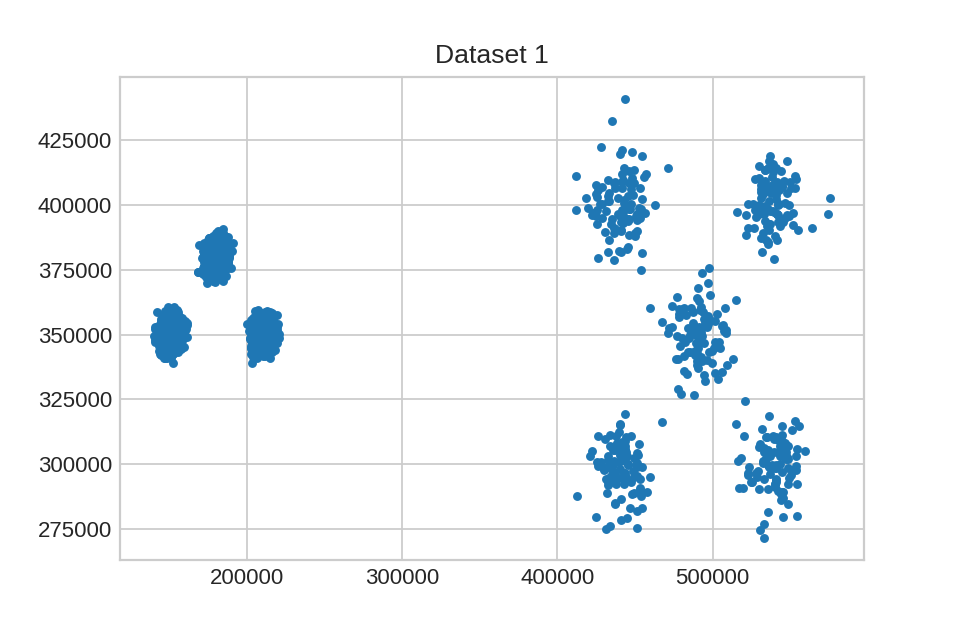
\includegraphics[scale=0.4]{experimentos/dataset1}
	\end{minipage}\qquad
	\begin{minipage}[t]{.3\textwidth}
		\centering
		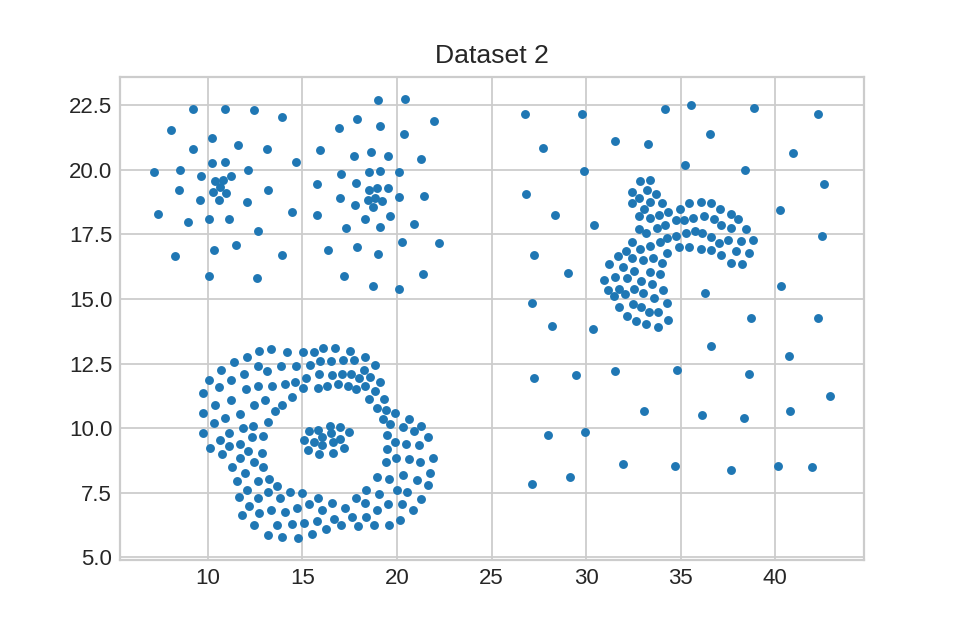
\includegraphics[scale=0.4]{experimentos/dataset2}
	\end{minipage}\qquad
	\begin{minipage}[t]{.3\textwidth}
		\centering
		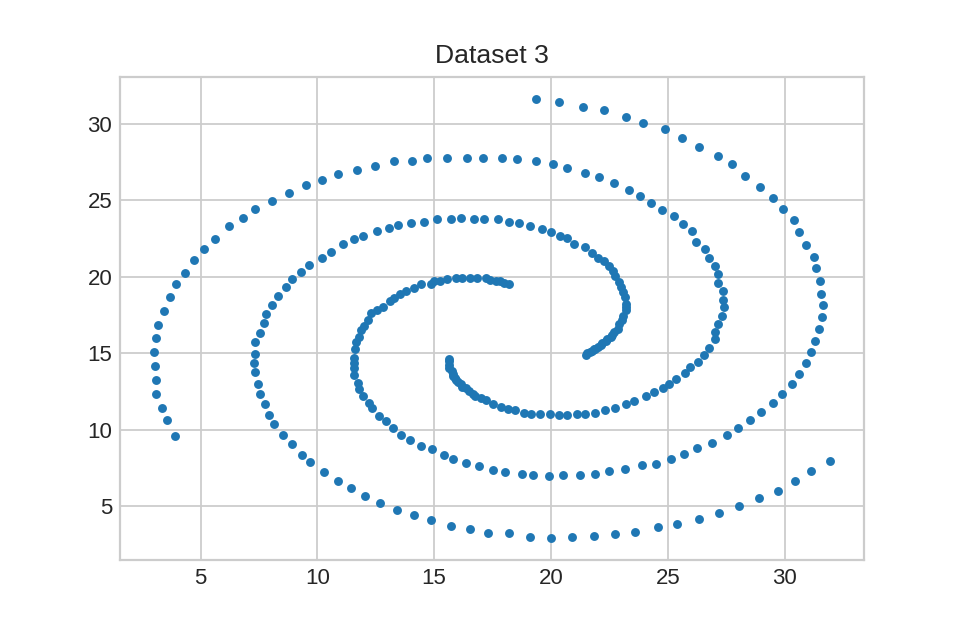
\includegraphics[scale=0.4]{experimentos/dataset3}
	\end{minipage}
\end{figure}	


\fbox{
	\parbox{0.9\textwidth}{
\textbf{Nota}: Para todos los criterios vamos a utilizar una profundidad de exploración fija de 9 ejes adyacentes. 
	}
}
\vspace{10 pt}

\subsubsubsection{Solo desvío estándar}
En este caso, vamos a descartar únicamente los ejes que son declarados inconsistentes al exceder en más de $\sigma$ veces el desvío estándar aplicado sobre el tamaño de eje promedio del vecindario.

\begin{figure}[H]
	\centering
	\begin{minipage}[t]{.3\textwidth}
		\centering
		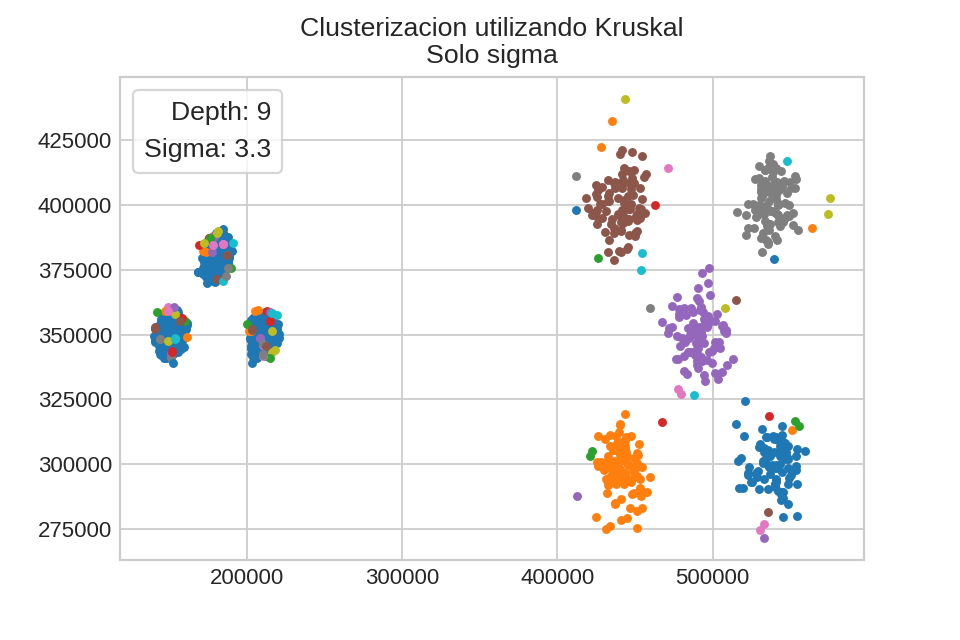
\includegraphics[scale=0.4]{experimentos/ds1-solosigma}
	\end{minipage}\qquad
	\begin{minipage}[t]{.3\textwidth}
		\centering
		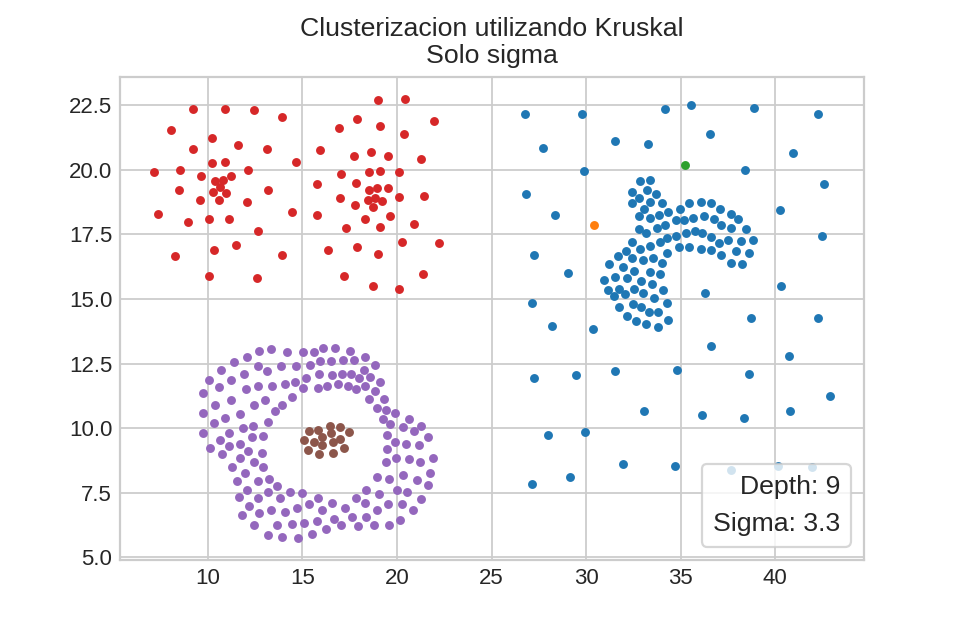
\includegraphics[scale=0.4]{experimentos/ds2-solosigma}
	\end{minipage}\qquad
	\begin{minipage}[t]{.3\textwidth}
		\centering
		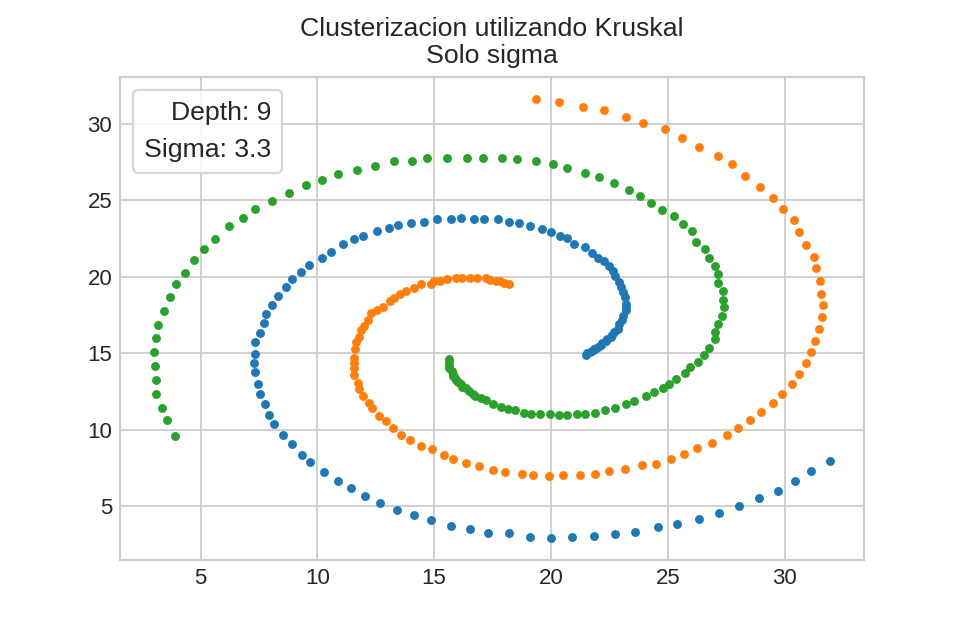
\includegraphics[scale=0.4]{experimentos/ds3-solosigma}
	\end{minipage}
\end{figure}	

Como podemos ver, utilizar solo el desvío estándar sirve para algunos casos, sin embargo tiene problemas para el \textit{dataset-1}, dado que en los clusters más chicos la desviación estándar entre los puntos es más alta, al estar todos más juntos. No podemos lograr un consenso de clusters sobre estos sin perjudicar la clusterización para los grupos de la derecha.


\subsubsubsection{Solo relación sobre el eje promedio}
En este caso, vamos a descartar únicamente los ejes que son declarados inconsistentes al ser $\digamma$ veces más grandes que el tamaño de eje promedio del vecindario.


\begin{figure}[H]
	\centering
	\begin{minipage}[t]{.3\textwidth}
		\centering
		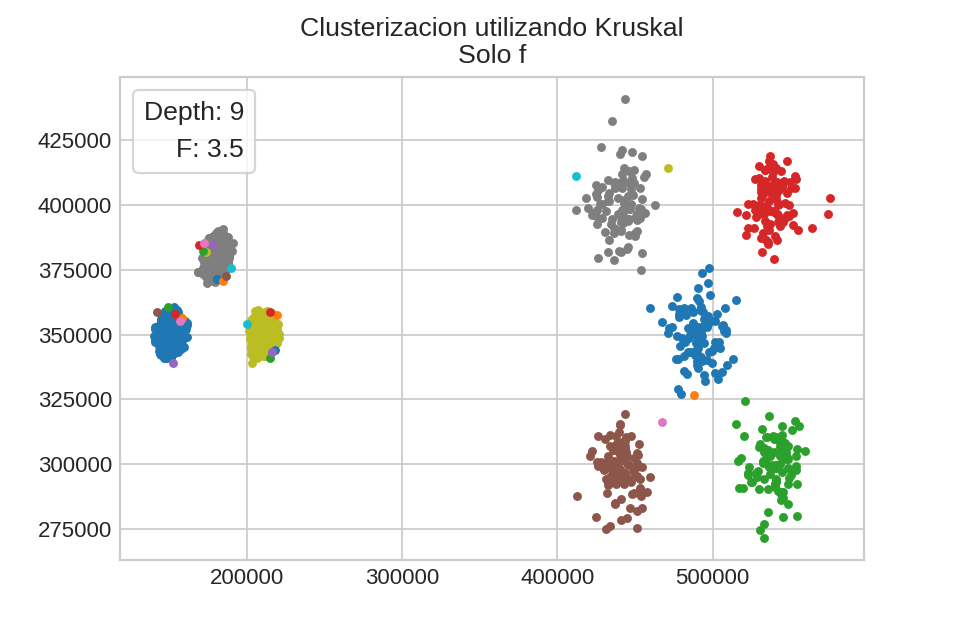
\includegraphics[scale=0.4]{experimentos/ds1-solof}
	\end{minipage}\qquad
	\begin{minipage}[t]{.3\textwidth}
		\centering
		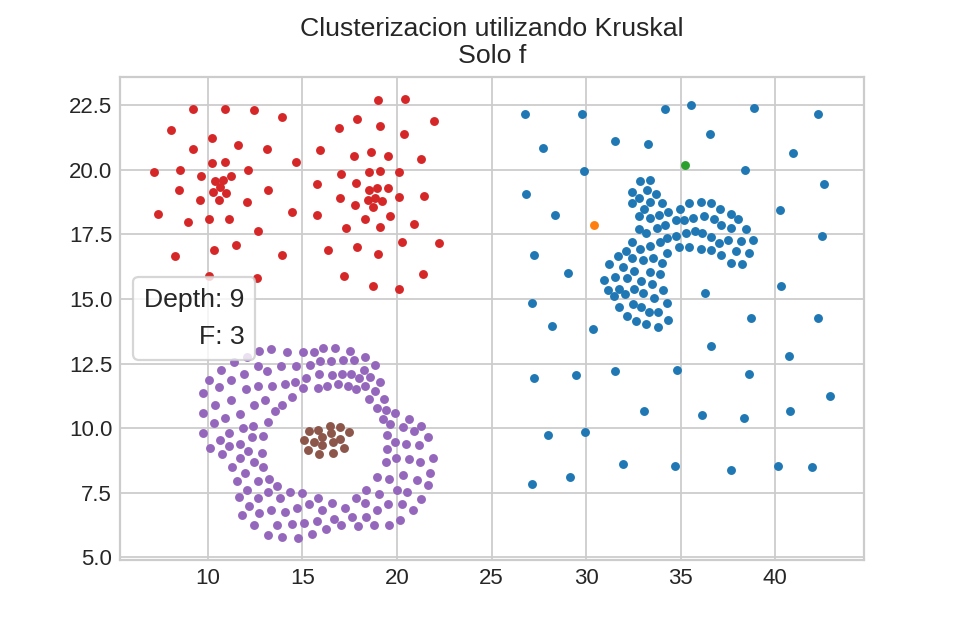
\includegraphics[scale=0.4]{experimentos/ds2-solof}
	\end{minipage}\qquad
	\begin{minipage}[t]{.3\textwidth}
		\centering
		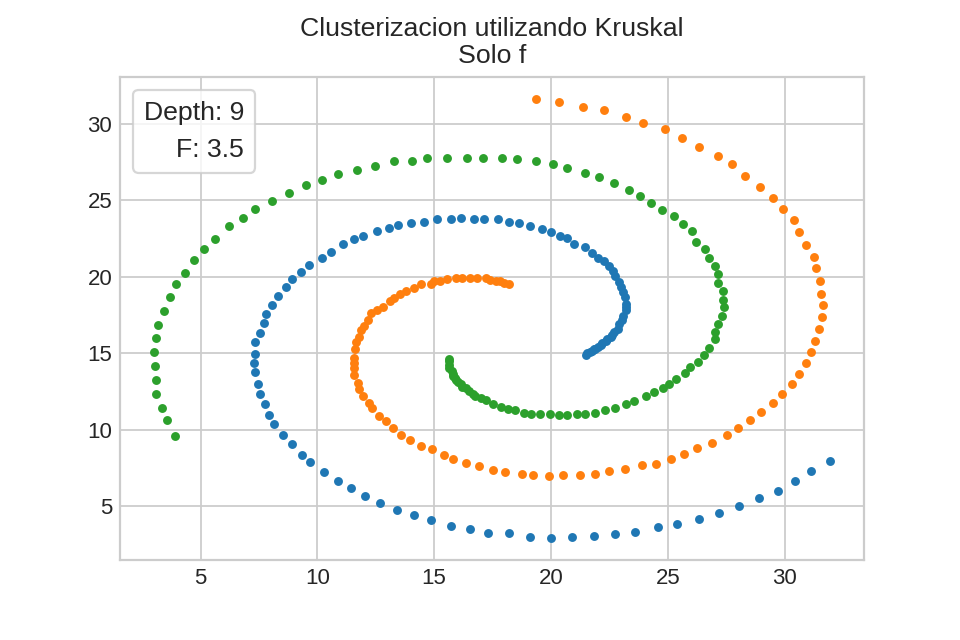
\includegraphics[scale=0.4]{experimentos/ds3-solof}
	\end{minipage}
\end{figure}

En este caso podemos ver que el \textit{dataset-1} no es problema para este criterio, aunque hay que notar que para el caso del \textit{dataset-2}, hubo que elegir un $f$ distinto, ya que los clusters de lado izquierdo eran agrupados con el valor utilizado para los otros datasets.

\subsubsubsection{Desvío estándar o relación de eje promedio}
Para este caso, los ejes inconsistentes van a ser los que cumplan con alguno de los dos criterios anteriores


\begin{figure}[H]
	\centering
	\begin{minipage}[t]{.3\textwidth}
		\centering
		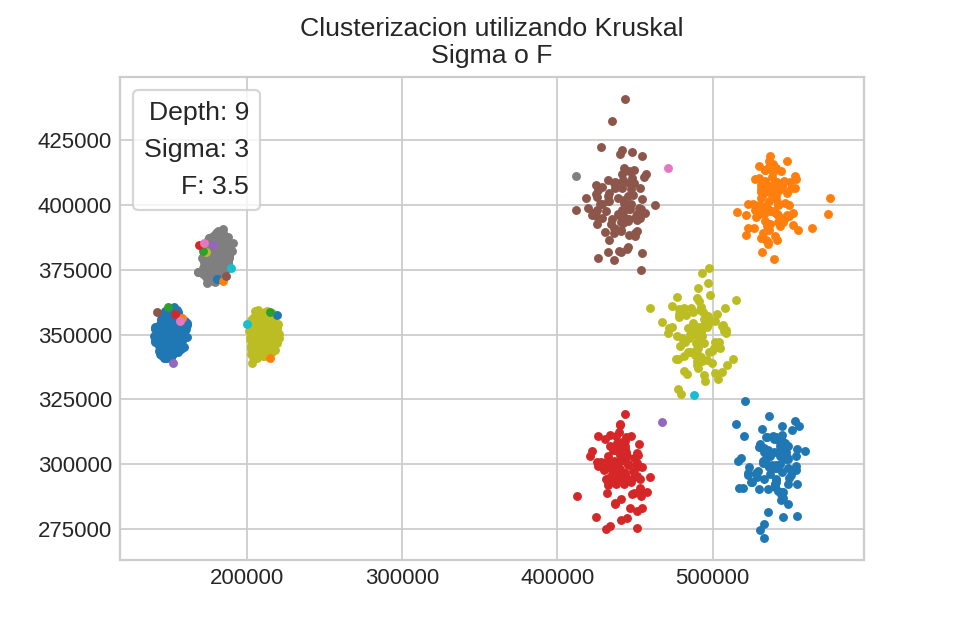
\includegraphics[scale=0.4]{experimentos/ds1-sigmaof}
	\end{minipage}\qquad
	\begin{minipage}[t]{.3\textwidth}
		\centering
		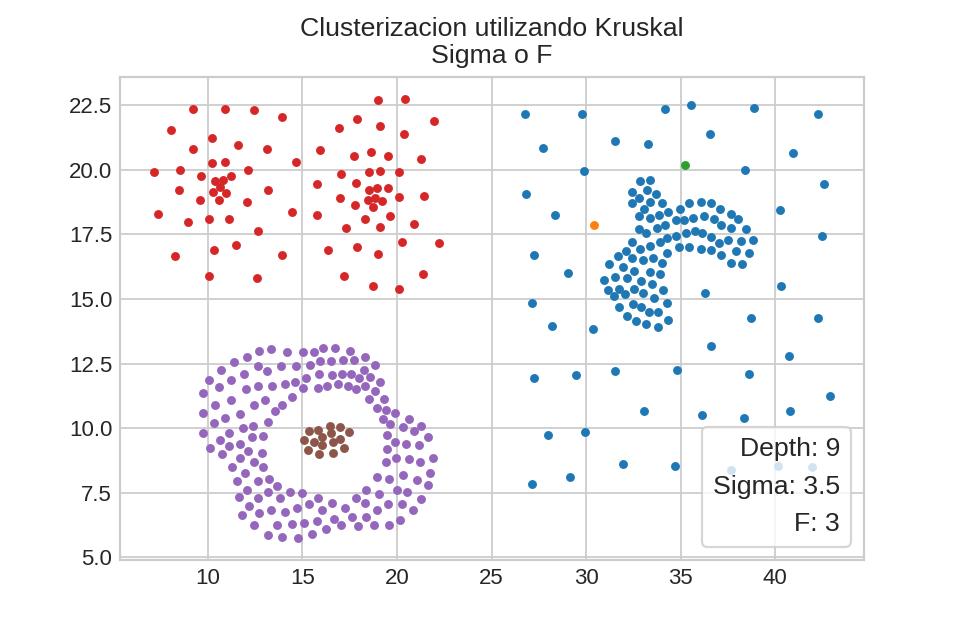
\includegraphics[scale=0.4]{experimentos/ds2-sigmaof}
	\end{minipage}\qquad
	\begin{minipage}[t]{.3\textwidth}
		\centering
		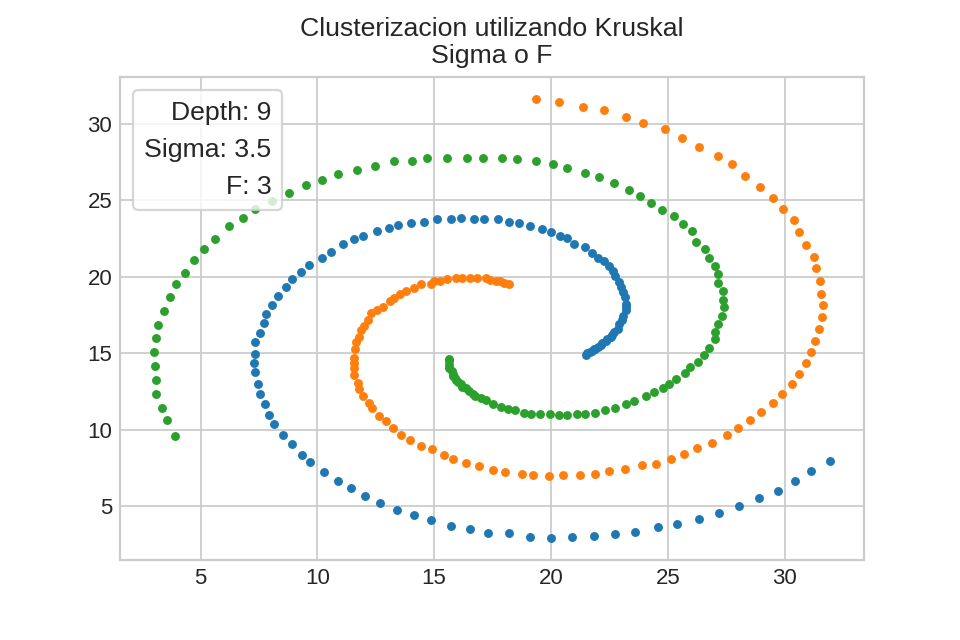
\includegraphics[scale=0.4]{experimentos/ds3-sigmaof}
	\end{minipage}
\end{figure}

Al utilizar cualquiera de los dos criterios anteriores para descartar nodos, podemos ver que en general toma precedencia el criterio por ‘f’ (relación de tamaño con el eje promedio). Por lo que no observamos beneficios al incluir el desvío estándar en la comparación. 

\subsubsubsection{Desvío estándar y relación de eje promedio}
Para este último caso, vamos a descartar únicamente los ejes que sean declarados inconsistentes tanto por el criterio del desvío estándar como por el criterio de relación de eje.

\begin{figure}[H]
	\centering
	\begin{minipage}[t]{.3\textwidth}
		\centering
		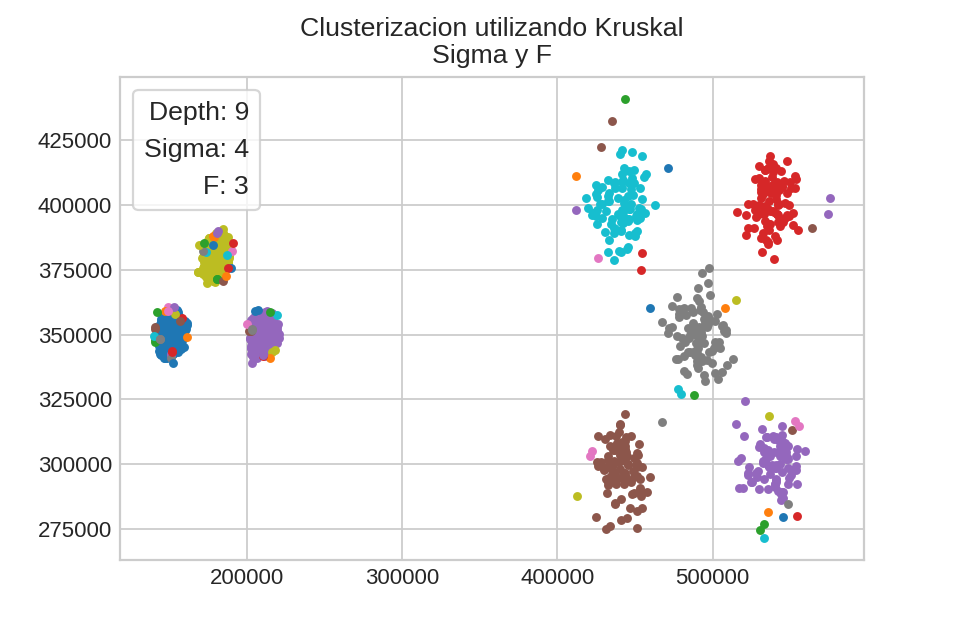
\includegraphics[scale=0.4]{experimentos/ds1-sigmayf}
	\end{minipage}\qquad
	\begin{minipage}[t]{.3\textwidth}
		\centering
		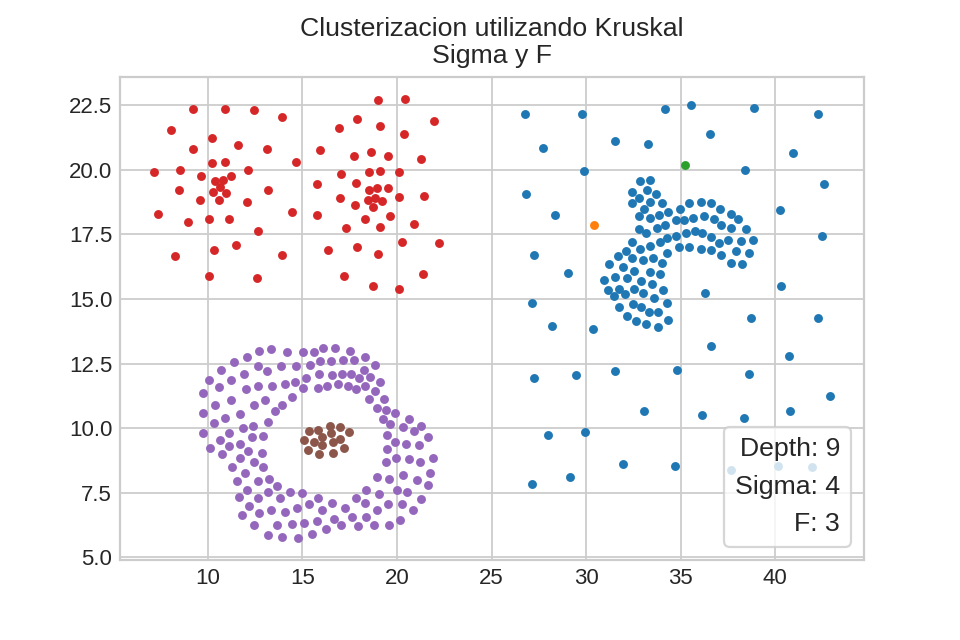
\includegraphics[scale=0.4]{experimentos/ds2-sigmayf}
	\end{minipage}\qquad
	\begin{minipage}[t]{.3\textwidth}
		\centering
		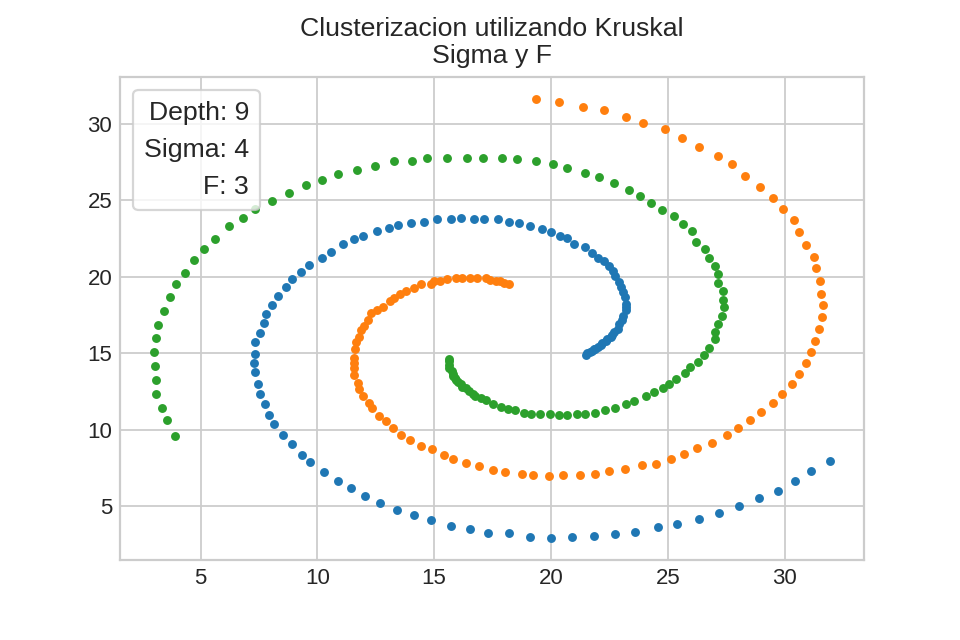
\includegraphics[scale=0.4]{experimentos/ds3-sigmayf}
	\end{minipage}
\end{figure}

Siguiendo el caso anterior, podemos ver que usar la conjunción sólo resulta en peores resultados, dado que para forzar la clusterización en algunos grupos, debemos usar un valor alto para sigma, lo cual resulta en agrupamientos indeseados en otras partes del grafo.

\subsubsubsection{Conclusiones}

Para los grafos elegidos para el experimento, resulta más conveniente utilizar únicamente la relación del eje contra el tamaño promedio de ejes. Como experimentos para profundizar, se deberían elegir grafos en los cuales la desviación estándar sea mayor al tamaño de eje promedio, en cuyo caso podríamos sacar provecho de combinar ambos criterios.


\subsubsection{Kruskal vs Kruskal con path compression}
Tal como fue presentado en la implementación del algoritmo de Kruskal, el mismo se puede implementar con un DSU con \textbf{path compression} que consiste en recordar el representante de un nodo buscado para poder accederlo en $\mathcal{O}(1)$ en la próxima consulta.

Para poder llevar a cabo dicha comparación, los escenarios planteados son representados con los siguientes grafos con 14600 puntos cada uno:

\begin{figure}[H]
	\centering
	\begin{minipage}[t]{.3\textwidth}
		\centering
		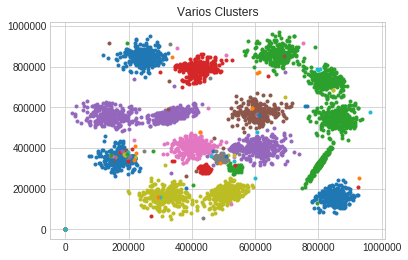
\includegraphics[scale=0.44]{experimentos/variosClusters}
	\end{minipage}\qquad
	\centering
	\begin{minipage}[t]{.3\textwidth}
		\centering
		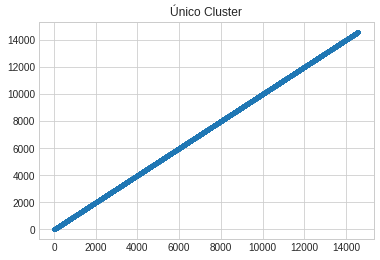
\includegraphics[scale=0.44]{experimentos/unicoCluster}
	\end{minipage}\qquad
\end{figure}	

\textbf{Nota}: Los puntos de la curva representan el promedio de ciclos de reloj de 10 ejecuciones por punto. Para cada grafo, desde 0 hasta 6500 se generaron datos en intervalos de 325 puntos, luego se genero información para 11500 puntos y por último para 14600 puntos.

\vspace{10 pt}

Los puntos a evaluar son:
\begin{itemize}
\item Performance entre Kruskal y Kruskal con path compression con varios clusters.
\item Performance entre Kruskal y Kruskal con path compression con un único cluster.
\item Evaluación de Kruskal con cota.
\end{itemize}


\subsubsubsection{Performance con varios clusters}


Al utilizar un grafo de 14600 puntos repartido en varios clusters como se pudo observar en la figura, se puede ver que cada cluster no contiene muchos puntos. Si bien, la alternativa de kruskal con path compression permite acceder al representante de un cluster en  $\mathcal{O}(1)$, al tratarse de clusters con pocos puntos, se espera que haya una diferencia mínima en los ciclos de reloj.

\begin{figure}[H]
	\centering
	\begin{minipage}[t]{.3\textwidth}
		\centering
		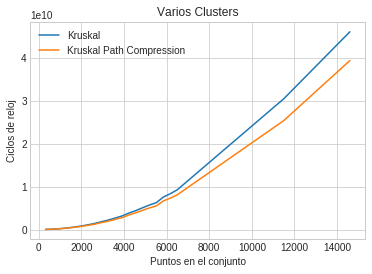
\includegraphics[scale=0.48]{experimentos/variosNormal}
	\end{minipage}
\end{figure}

Si bien la cantidad de ciclos de reloj entre una implementación y la otra comienzan a distanciarse a medida que se incrementan los puntos, la diferencia es mínima y se puede comprobar que la implementación con path compression se resuelve en menos ciclos.


\subsubsubsection{Performance con un único cluster}

Al utilizar el grafo de 14600 puntos repartido en un único cluster se espera que la optimización de path compression sea más visible y haya una mayor diferencia en la ejecución de cada algoritmo. 

\begin{figure}[H]
	\centering
	\begin{minipage}[t]{.3\textwidth}
		\centering
		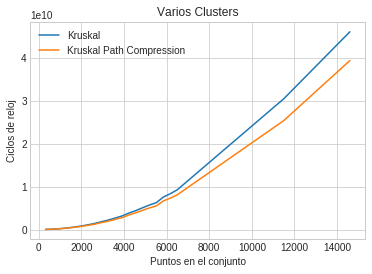
\includegraphics[scale=0.48]{experimentos/variosNormal}
	\end{minipage}
\end{figure}

Como se puede observar en la figura, los ciclos de reloj para cada algoritmo se distancian con una mayor diferencia que el caso anterior. Esto se debe a que la implementación normal de kruskal debe recorrer todo el arreglo de representantes, equivalente a recorrer todos los puntos ya analizados, para obtener el representante del cluster, que es único. En cambio, en el grafo anterior, los clusters contenían menos puntos, por ello la diferencia no era tan notable. En la última parte del grafo es posible ver como la pendiente de la ejecución para kruskal crece más rapidamente que para kruskal con path compression.


\subsubsubsection{Evaluación de cota}

La complejidad de ambas implementaciones es la misma, por eso se espera que ante la cota tomada, ambos pasen a estar por debajo de la misma a partir de un cierto valor.

\begin{figure}[H]
	\centering
	\begin{minipage}[t]{.3\textwidth}
		\centering
		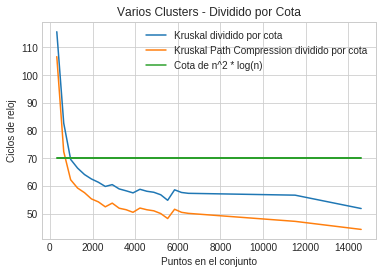
\includegraphics[scale=0.44]{experimentos/variosDivididoPorCota}
	\end{minipage}
	\centering
	\begin{minipage}[t]{.3\textwidth}
		\centering
		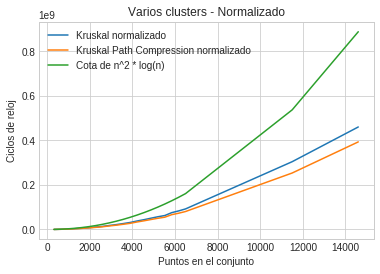
\includegraphics[scale=0.44]{experimentos/variosNormalizadoCota}
	\end{minipage}
\end{figure}

Como podemos ver, la funcion converge a un valor constante al dividirla por la complejidad planteada, lo cual demuestra que cumple con dicha cota.
\subsubsection{Comparacion de Kruskal contra Prim}

Al comparar Prim y Kruskal a la hora de clusterizar, podemos ver que ambos producen resultados similares. La diferencia entre ambos existe a la hora de generar el árbol generador mínimo, sobre el cual luego se descartan los ejes inconsistentes.

\begin{figure}[H]
	\centering
	\begin{minipage}[t]{.3\textwidth}
		\centering
		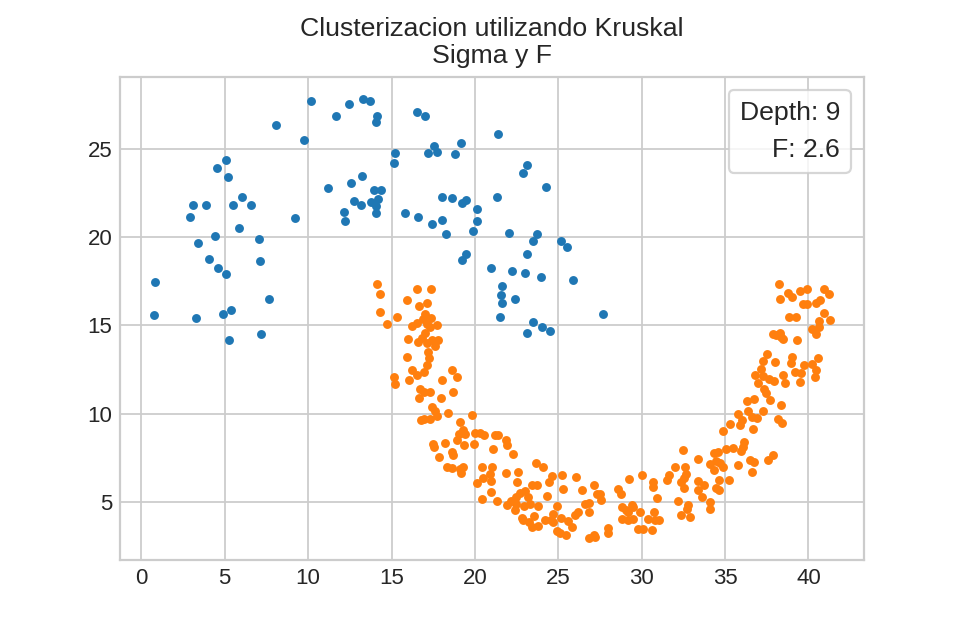
\includegraphics[scale=0.4]{experimentos/kvp-dataset-11-Kruskal}
	\end{minipage}\qquad
	\begin{minipage}[t]{.3\textwidth}
		\centering
		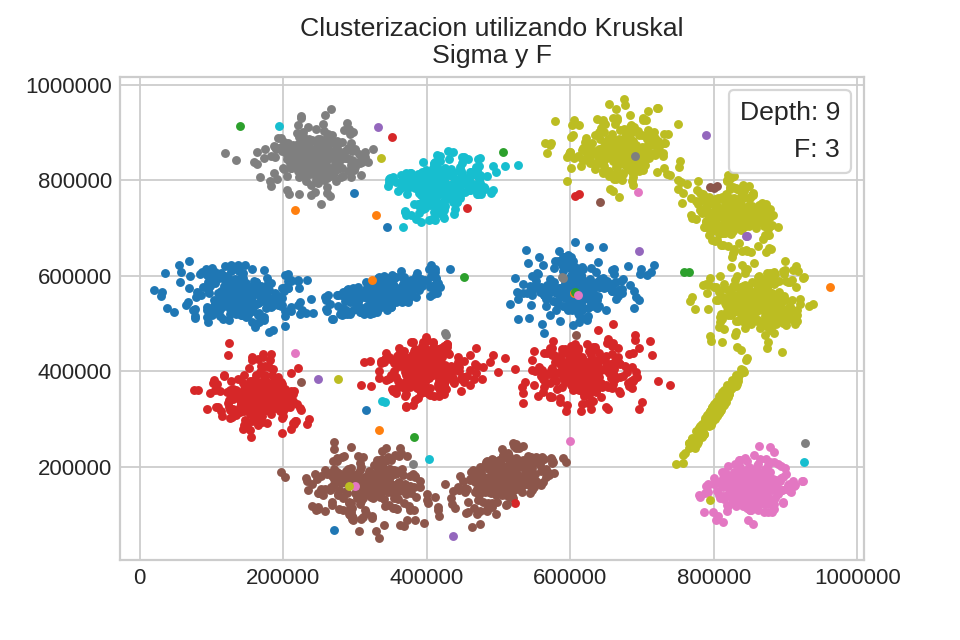
\includegraphics[scale=0.4]{experimentos/kvp-dataset-4-Kruskal}
	\end{minipage}\qquad
	\begin{minipage}[t]{.3\textwidth}
		\centering
		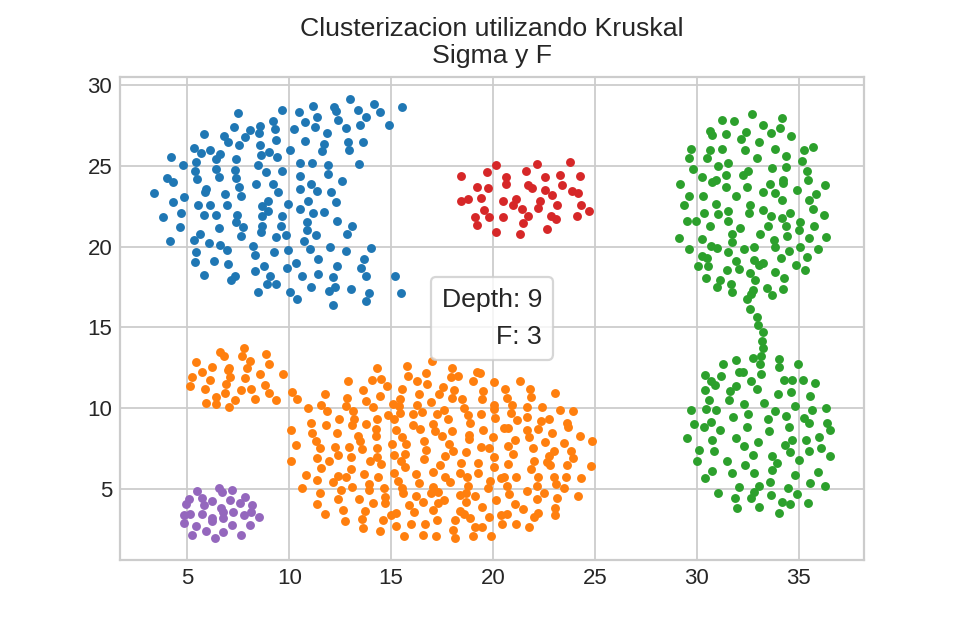
\includegraphics[scale=0.4]{experimentos/kvp-dataset-6-Kruskal}
	\end{minipage}
\end{figure}	

\begin{figure}[H]
	\centering
	\begin{minipage}[t]{.3\textwidth}
		\centering
		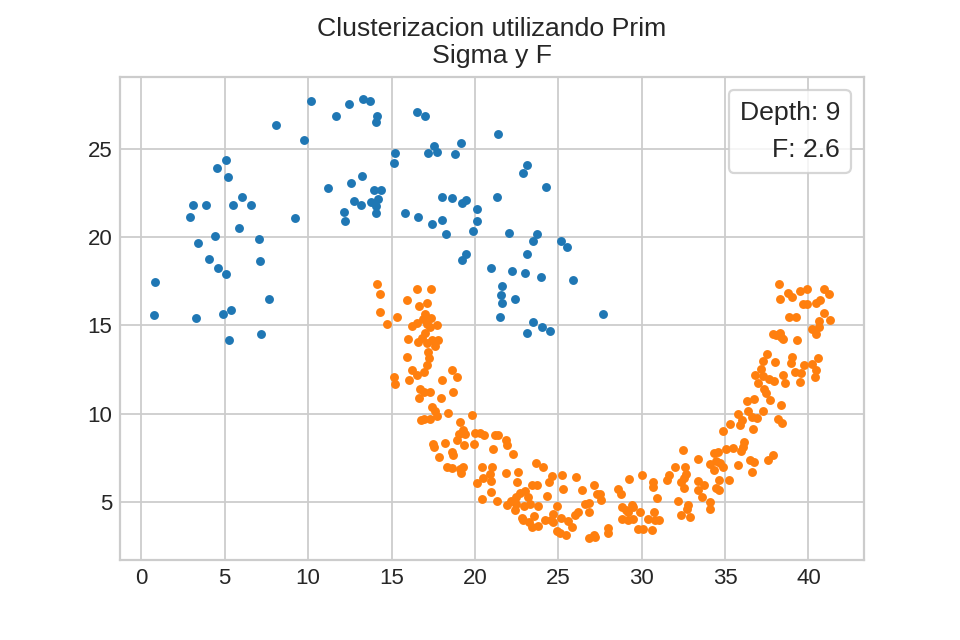
\includegraphics[scale=0.4]{experimentos/kvp-dataset-11-Prim}
	\end{minipage}\qquad
	\begin{minipage}[t]{.3\textwidth}
		\centering
		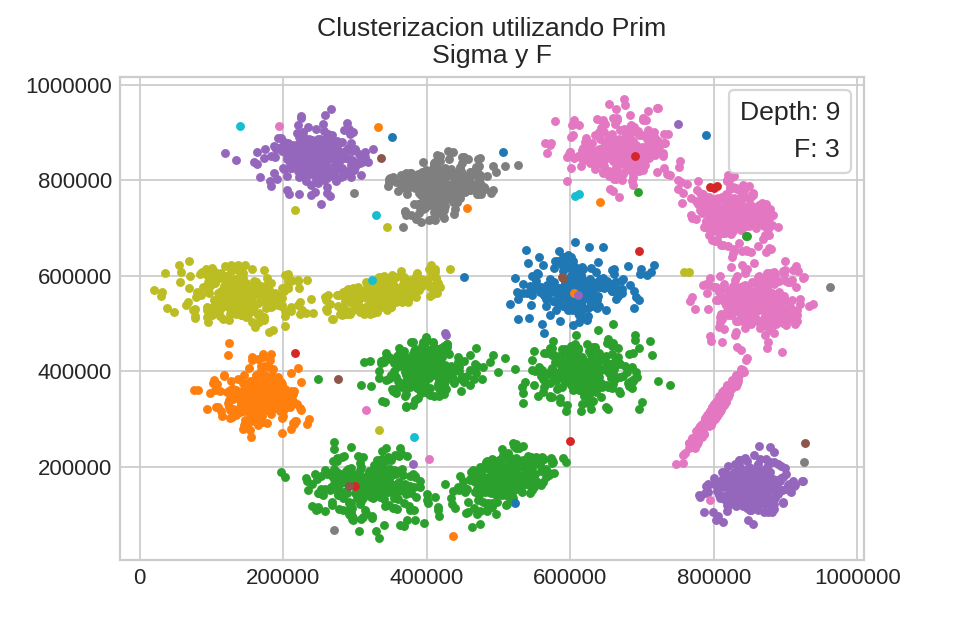
\includegraphics[scale=0.4]{experimentos/kvp-dataset-4-Prim}
	\end{minipage}\qquad
	\begin{minipage}[t]{.3\textwidth}
		\centering
		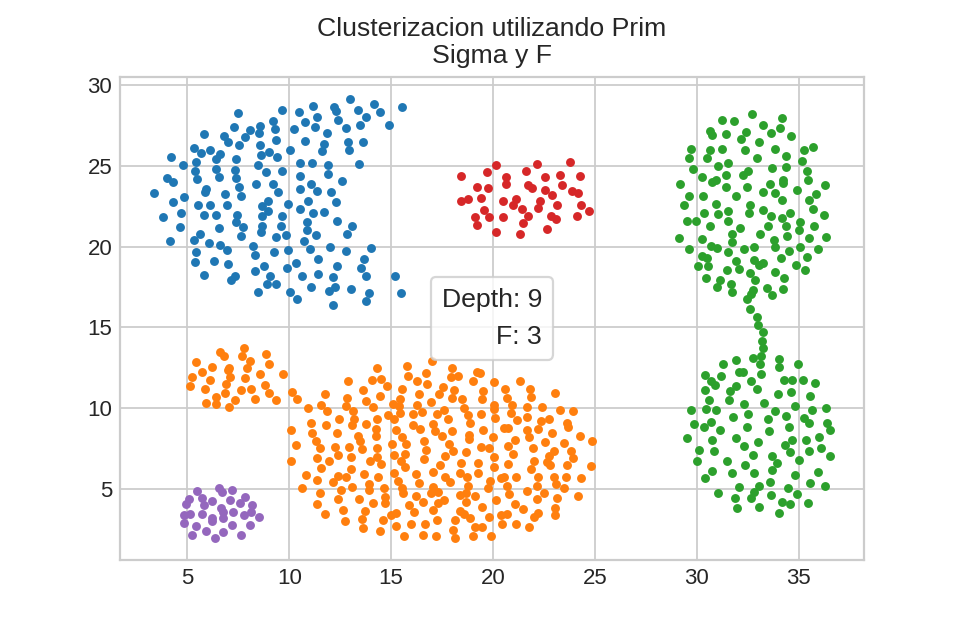
\includegraphics[scale=0.4]{experimentos/kvp-dataset-6-Prim}
	\end{minipage}
\end{figure}	

\subsubsubsection{Conclusiones}

Sin embargo, cabe destacar para Kruskal -al ser un algoritmo bottom up- armar los clusters una vez recortado el árbol generador mínimo es una tarea trivial, ya que el algoritmo se basa en formar clusters desconectados. En este aspecto, debemos realizar una solución Ad-Hoc para Prim, lo cual nos fuerza a obtener una complejidad mayor, a fuerza de no implementar Kruskal para clusterizar dentro de Prim.

\begin{figure}[H]
	\centering
	\begin{minipage}[t]{.45\textwidth}
		\centering
		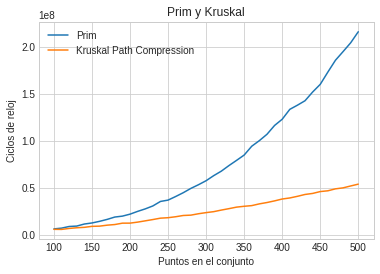
\includegraphics[scale=0.55]{experimentos/prim-v-kruskal}
	\end{minipage}\qquad
	\begin{minipage}[t]{.45\textwidth}
		\centering
		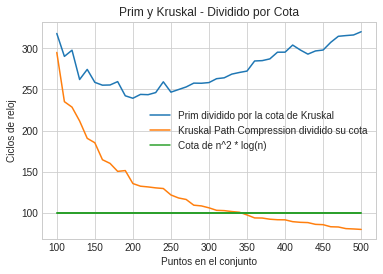
\includegraphics[scale=0.55]{experimentos/prim-v-kruskal-acotado}
	\end{minipage}
\end{figure}	


\subsection{Conclusiones}

\subsubsection{Analisis Comparativo entre los Algoritmos} \label{analisisComparativo}

La problematica de arbitraje fue resuelta con los algoritmos de Bellman-Ford y Floyd-Warshall como mostramos en las secciones anteriores. Sabemos que la complejidad de Bellman-Ford es $\mathcal{O}(nm)$. Si tenemos en cuenta que en este problema de arbitraje necesitamos el camino minimo entre todo par de nodos, debemos ejecutar el algoritmo otras $`$n' veces, lo cual resulta en una complejidad de $\mathcal{O}(n^{2}m)$. Por otro lado, sabemos que la complejidad de Floyd-Warshall $\mathcal{O}(n^{3})$.

Esto nos dice que Bellman-Ford no tiene un buen caso en grafos completos, que es el caso del arbitraje. Floyd-Warshall no es afectado por grafos completos, pero si por el tamaño del mismo. Esto tiene relevancia dado que la experimentación ejecutada mostraba al algoritmo de Floyd como un claro ganador en tiempo. Es cierto que la implementación de Bellman-Ford no esté en el $\%$100 de su efectividad, pero es de esperar que en un grafo completo, Floyd-Warshall se comporte mejor.

Con respecto a los casos donde puede convenir uno u otro, vimos que ambos pueden ser utilizados para detectar un ciclo negativo. Floyd-Warshall es superior si el arbitraje se encuentra entre los primeros nodos, Bellman-Ford si no lo hay.

\section{Arbitraje}
\subsection{Introducción a la problemática}
% descripcion del problema
% algoritmos propuestos para resolverlo
% Bellman-Ford
% Floyd-Warshall

\subsubsection{Noción de arbitraje}
En finanzas, se denomina arbitraje a la práctica de comprar y vender un recurso de manera simultanea para generar una ganancia, aprovechandose de los desbalances de los precios en diferentes mercados. Supongamos que existe un recurso R disponible para la compra y venta en dos distintos mercados, $M_{1}$ y $M_{2}$.
 \par
En $M_{1}$, se puede comprar R por 42 pesos y vender por 41.8.
 \par
En $M_{2}$, se puede comprar R por 42,5 pesos y vender por 40,9.
 \par
Comprar en el segundo mercado para venderlo en el primero, o viceversa, no genera ganancia. Sin embargo, si el recurso se valoriza y $M_{1}$ se entera de este suceso: actualizará su cotización. De esta forma, ahora $M_{1}$ compra por 42,8 pesos el recurso y lo vende por 43,5. Hay oportunidad de arbitraje ya que $M_{2}$ no actualizó sus precios: por cada unidad comprada en $M_{2}$ y vendida en $M_{1}$ se obtiene 43,5-42,5 = 1 peso. 

\subsubsection{Arbitraje de divisas}
El problema a resolver en este trabajo es analizar si existe oportunidad de arbitraje entre varias divisas (pesos, dolares, euros, etc). Para ello, contamos con la tasa de cambio para cada divisa.

La entrada consistirá de un primer entero $n$ que corresponde a la cantidad de divisas a tener en cuenta. Luego, habrá $n$ líneas. Cada una de ellas tendrá $n$ numeros reales $c_{i,j}$, representando el multiplicador que se debe aplicar a una unidad de la divisa $i$ al cambiar a la divisa $j$. Si el arbitraje existe, la salida debe ser un posible ciclo de divisas, donde cada numero representará desde la divisa $0$ a la $n-1$.

A continuación se presentan dos ejemplos, uno donde existe arbitraje y otro donde no.
\begin{table}[!htb]
\begin{minipage}{.5\linewidth}
\begin{center}
	\begin{tabular}{ |l l l l|l| } 
		\hline
		&Entrada& de& ejemplo & Posible salida \\
		\hline
		4 &&&& 3 2 1 3 \\
		1& 0.1& 5& 0.125 & \\ 
		10& 1& 0.5& 0.3  & \\ 
		0.2& 2& 1& 2 & \\ 
		8& 3& 0.5& 1 & \\ 
		\hline
	\end{tabular}
\end{center}
\end{minipage}
\begin{minipage}{.5\linewidth}
\begin{center}
	\begin{tabular}{ |l l l l|l| } 
		\hline
		&Entrada& de& ejemplo & Salida\\
		\hline
		4 &&&& NO \\
		1& 0.1& 0.05& 0.125 & \\ 
		0.1& 1& 0.5& 0.3  & \\ 
		0.2& 0.02& 1& 0.2 & \\ 
		0.8& 0.3& 0.5& 1 & \\ 
		\hline
	\end{tabular}
\end{center}
\end{minipage}
\end{table}
%En el ejemplo de arriba, el ciclo es $\{2, 3, 1, 2\}$  ya que $c_{23}$ x $c_{31}$ x $c_{12}$ x $c_{21} = 3 > 1$
\par
Por lo tanto, debemos hallar una secuencia de divisas tal que al convertir una unidad de la divisa inicial a través de las monedas, se genere una ganancia. Esto se traduce a encontrar una secuencia S 
\begin{align*}
S =& \{d_a, d_b, d_c, ... , d_k\}\quad \text{tal que} \quad c_{a,b} \: \text{x} \: c_{b,c} \: \text{x ... x} \: c_{k,a} > 1 
\end{align*}
\par
En la entrada de ejemplo con solucion, un posible ciclo es $\{3, 2, 1, 3\}$  ya que $c_{32}$ x $c_{21}$ x $c_{13}$ = 2 x 10 x 5 = 100 $>$ 1.


\subsection{Análisis del problema} 
\subsubsection{Traduciendo a grafos}

\subsection{Bellman-Ford}
\subsubsubsection{Resolución} \label{res-bell}
Para resolver arbitraje usando Bellman Ford (\textbf{BF}) utilizamos una variación (\textbf{BF'}) del algoritmo clásico. \textbf{BF'} considera la \textit{longitud} de un camino como el \textit{producto} de sus aristas, y busca \textit{maximizar} (y no minimizar) la longitud. Utilizamos esta variación ya que es la más natural dada el input que recibimos: si queremos pasar de un activo $i$ a un activo $j$, tenemos que  multiplicar por $c_{i,j}$ y no sumar. En esta variación del algoritmo, un arbitraje será un ciclo tal que el producto de sus aristas sea estrictamente mayor a $1$.

\begin{algorithm}[H]
\caption{Find arbitrage}
\begin{algorithmic}[1]
\Function{Bellman-Ford'}{$vector<Nodo> nodos$, $vector<Eje> ejes$, $Nodo$ $inicial$}
	\State \textbf{Inicializar}
	\State $\pi = vector<int>$[$number\_of\_nodes$]
	\State $predecesor = vector<int>$[$number\_of\_nodes$]
	\For{$u \in nodos$}
		\State $\pi(u) = 0$
		\State $predecesor(u) = -1$
	\EndFor
	\State $\pi(inicial) = 1$
	\Statex								
	\For{$i=0; i \leq number\_of\_nodes; i++$} 													
		\For{$e \in ejes$}
			\If{$\pi(e.terminal) < \pi(e.comienzo) * e.peso$}
				\State $\pi (e.terminal)=e.comienzo * e.peso$
				\State $predecesor (e.terminal) = e.comienzo$
			\EndIf		
		\EndFor
	\EndFor
	\Statex
	\For{$e \in ejes$} 													
		\If{$\pi(e.terminal) < \pi(e.comienzo) * e.peso$}
			\State $vector<int> ciclo = \textbf{reconstruir_arbitraje}$
			\State \Return $ciclo$
		\EndIf
	\EndFor
	\Statex
	\State \Return $NO$
\EndFunction
\end{algorithmic}
\end{algorithm}

\subsubsubsection{Justificacion}
Podemos ensayar una justificación de porqué el algoritmo funciona apoyándonos en el homeomorfismo monótono decreciente $e^{-x} :(\mathbb{R}, +) \longrightarrow (\mathbb{R}_{>0}, .) $ y su inversa $-log(x) : (\mathbb{R}_{>0}, .) \longrightarrow (\mathbb{R}, +)$:

Sea $(G,I)$ tal que $I(w,u) > 0 \forall (w,u)$. Este es el problema original que recibiremos, donde los pesos de las aristas es cuanto cuesta el cambio de un activo a otro. Defino $\tilde{G} = (G, -log(I))$, osea aplico $-log$ a los pesos. Sea $\tilde{\pi}$ una solución clásica de $BF$. Notar que la condición de que $\tilde{G}$ no tenga ciclos de longitud negativa alcanzables desde $v$ es equivalente a que $G$ no tenga ciclos de \textit{longitud} (productoria) estrictamente mayor a 1 alcanzables desde 1 (es decir, que haya un arbitraje). 

Sea ahora $C$ un camino de $v$ a $u_0$. Entonces por def. de solución de $BF$,

$$ \tilde{\pi}(u_0) \leq l(C) = \sum \tilde{I} (a_i, a_{i+1}) = - \sum log(I(a_i, a_{i+1}))$$

Aplicando $e^{-x}$,
$$ e^{-\tilde{\pi}(u_0)} \geq e^{ - ( - \sum logI(a_i, a_{i+1}) )} = e^{ \sum logI(a_i, a_{i+1})}$$
Si defino $\pi$ como $e^{-\tilde{\pi}}$, tengo que
$$\pi (u_0) \geq \prod I(a_i , a_{i+1})$$

Es decir, obtenemos una solución que maximiza los productos. Esto demuestra que pudimos haber hecho $BF$ tradicional en $(G, -log(I))$, y al resultado aplicarle $e^{-x}$ (coordenada a coordenada) para obtener una solución del problema de maximizar con el producto. Por otra parte, si tomamos el algoritmo de $BF'$ como aparece en el pseudo-código y ''aplicamos'' la función $-log$, usando que $"-log(0)" = +\infty$ y que el resultado de aplicar $-log$ a 
$$\pi(e.terminal) < \pi(e.comienzo) * e.peso$$
es
\begin{align}
    -log(\pi(e.terminal)) &\geq -log(\pi(e.comienzo)) + - log( e.peso) \\        
    \tilde{\pi}(e.terminal) &\geq \tilde{\pi}(e.comienzo) + \tilde{\pi}(e.peso)
\end{align}

Es decir, intuitivamente, podemos transformar el algoritmo modificado ($BF'$) y obtener el BF tradicional, que sabemos que funciona (porque ya lo demostramos). Pero también podemos volver con $e^-x$ y obtener el algoritmo original ($BF'$). Por lo tanto $BF'$ también funciona. Si bien intuitivamente es claro que la correspondencia entre $-log(x) y e^-x$ hace que la modificación del algoritmo funcione, no es formal. Una demostración formal podría hacerse por ejemplo copiando la demostración de $BF$ clásica y reemplazando $+$ por $.$, $<$ por $\geq$ y haciendo los cambios correspondientes.
\subsection{Floyd-Warshall}
\subsubsubsection{Resolución} \label{res-floyd}
El algoritmo de Floyd-Warshall es un algoritmo matricial que calcula la distancia entre todos los distintos nodos. Dado que la entrada del ejercicio es la matriz de tipos de cambio, podemos tomar a la misma como la matriz de entrada para el algoritmo, llamemosla L. Donde cada $`$i', $`$j' de la matriz representa el peso de la arista desde el nodo $`$i' a $`$j'. Sea l(ij) la funcion que define este peso.

Como parte del ejercicio es devolver el ciclo de arbitraje encontrado, debemos tener una manera de reconstruir dicho ciclo. Para ello, utilizaremos la matriz $``$next", una matriz de sucesores, que tiene el mismo tamaño que la matriz de entrada. La matriz $``$next" es inicializada con cada nodo indicando a si mismo como su sucesor.

Una vez que tenemos la matriz de sucesores, procedemos a resolver el camino máximo del grafo. Para ello, el algoritmo de Floyd-Warshall recurre a tres ciclos anidados donde recorremos la matriz. La idea es trabajar con una matriz $``$virtual" representada en la iteracion del ciclo principal, que llamaremos $`$k'. Los otros dos ciclos recorren el valor de $`$i' en el primer caso y el de $`$j' en el ciclo interno. Por cuestiones de complejidad temporal, Floyd-Warshall nos permite siempre trabajar sobre la matriz inicial, sin necesidad de crear una nueva para cada paso. En cada paso del ciclo $`$k', que itera el valor de $`$k' entre 0 y $`$n', el algoritmo calcula el camino máximo de un vertice $`$i' a otro $`$j' con vertices intermedios en el conjunto $``${0,....,k}".

$L^{k}$ es la matriz del paso $`$k'. Lo cual nos permite la siguiente definicion:

- $L^{0}[i][j]$ = 0 y para i$neq$j, $L^{0}[i][j]$ = l(ij) si ij pertence a los ejes del grafo. En este caso, el grafo es completo asi que el eje siempre existe.

- $L^{k+1}[i][j]$ = max{$L^{k}[i][j]$, $L^{k}[i][k]$ * $L^{k}[k][j]$}. Esta funcion no es la original del algoritmo de Floyd-Warshall, ya que aquí buscamos maximizar la longitud del camino. Esto es válido de la misma forma que la variante de Bellman-Ford presente en este trabajo práctico. Podemos encontrar la justificación de la utilización del producto en la sección 2.2.0.2, es decir, la misma justificación que Bellman-Ford. En este paso, tambien actualizamos el valor de la matriz de sucesores en caso de que el valor maximo sea el del segundo argumento. En dicho caso, como el camino del nodo $`$i' a $`$j' necesita pasar primero por el nodo $`$k', podemos decir que el camino es igual al camino de $`$i' a $`$k'.

La matriz buscada es $L^{n}$.

Al final de cada iteracion del ciclo $`$j', el algoritmo verifica si el elemento en la posicion $[i][i]$ es mayor a 1. Esto es equivalente a buscar si se formo el ciclo de arbitraje. Esto se hace al final de cada iteracion de $`$j' porque significa que ya actualizamos la distancia del nodo $`$i' a todos los demas, por eso queremos ver si en esta modificacion obtuvimos un ciclo de arbitraje. Al encontrar dicho ciclo pasamos a reconstruir el mismo, en caso de que no se encuentre, el algortimo habra iterado los tres ciclos por completo. Como $`$k', $`$i' y $`$j' iteran entre 0 y $`$n', iterar los tres por completo nos presenta la complejidad $\mathcal{O}(n^{3})$ del algoritmo.

Reconstruir el ciclo solo nos presenta complejidad $\mathcal{O}(n)$. El mismo recorre el camino formado en la matriz de sucesores. Tomamos como punto de partida el nodo $next[i][i]$. Obteniendo ese valor, que llamaremos $`$suc', lo que queremos es pedir el siguiente del nodo $[suc][i]$, para reconstruir el camino desde el sucesor ($`$suc') hasta $`$i' nuevamente.

\begin{algorithm}[H]
	\caption{arbitraje(Matriz cotizaciones, int n) res: vector<int> cicloArbitraje}
	\begin{algorithmic}[1]
		\State $vector<int> cicloArbitraje$ \Comment $\mathcal{O}(n)$
		\State $Matriz<int, int> sucesores \gets getNextElementMatrix(n)$ \Comment $\mathcal{O}(n^{2})$
		\For{$k = 0, n$} \Comment $\mathcal{O}(n^{3} + n)$
			\For{$i = 0, n$}
				\For{$j = 0, n$}
					\State $distanciaCalculada \gets cotizaciones[i][k] * cotizaciones[k][j]$
					\If{$cotizaciones[i][j] < distanciaCalculada$}
						\State $cotizaciones[i][j] \gets distanciaCalculada$
						\State $sucesores[i][j] \gets sucesores[i][k]$
					\EndIf
				\EndFor
				\If{$cotizaciones[i][j] > 1$}
					\State \textbf{return} $computeArbitrajeCycle(sucesores, i)$
				\EndIf
			\EndFor
		\EndFor
		\State \textbf{return} $cicloArbitraje$
	\end{algorithmic}
\end{algorithm}


\begin{algorithm}[H]
	\caption{getNextElementMatrix(int n) res: Matriz sucesores}
	\begin{algorithmic}[1]
		\State $Matriz<int, int> sucesores$
		\For{$i = 0, n$} \Comment $\mathcal{O}(n^{2})$
			\For{$j = 0, n$}
				\State $sucesores[i][j] \gets j$
			\EndFor
		\EndFor
		\State \textbf{return} $sucesores$
	\end{algorithmic}
\end{algorithm}


\begin{algorithm}[H]
	\caption{computeArbitrajeCycle(Matriz sucesores, int i) res: Matriz sucesores}
	\begin{algorithmic}[1]
		\State $vector<int> cicloArbitraje$
		\State $suc \gets sucesores[i][i]$
		\State $cicloArbitraje.push_back(i)$
		\While{$suc \neq i$} \Comment $\mathcal{O}(n)$
			\State $cicloArbitraje.push_back(suc)$
			\State $suc \gets sucesores[r][i]$
		\EndWhile
		\State $cicloArbitraje.push_back(i)$
		\State \textbf{return} $sucesores$
	\end{algorithmic}
\end{algorithm}
\subsection{Experimentación}

\subsubsection{Criterios para evaluación de ejes}
Al momento de decidir que ejes van a ser considerados inconsistentes (y por ende descartados), es necesario utilizar un criterio que se adapte a los diversos escenarios posibles.
\textbf{Charles Zahn} propone utilizar el desvío estándar y la relación al tamaño de eje promedio para esto.

En esta sección vamos a explorar cuál composición de criterios se adaptan mejor a los distintos tipos de clusters. Las opciones a comparar son:

\begin{itemize}
\item Utilizar solo el desvío estándar
\item Utilizar solo la relación al tamaño de eje promedio
\item Utilizar el desvío estándar O la relación al eje promedio
\item Utilizar el desvío estándar Y la relación al eje promedio
\end{itemize}

Para realizar las comparaciones vamos clusterizar los siguientes 3 grafos, definiendo como mas optimo al criterio que mejor arme clusters en todos los escenarios utilizando la menor cantidad de esfuerzo en elección de parámetros posible.

\begin{figure}[H]
	\centering
	\begin{minipage}[t]{.3\textwidth}
		\centering
		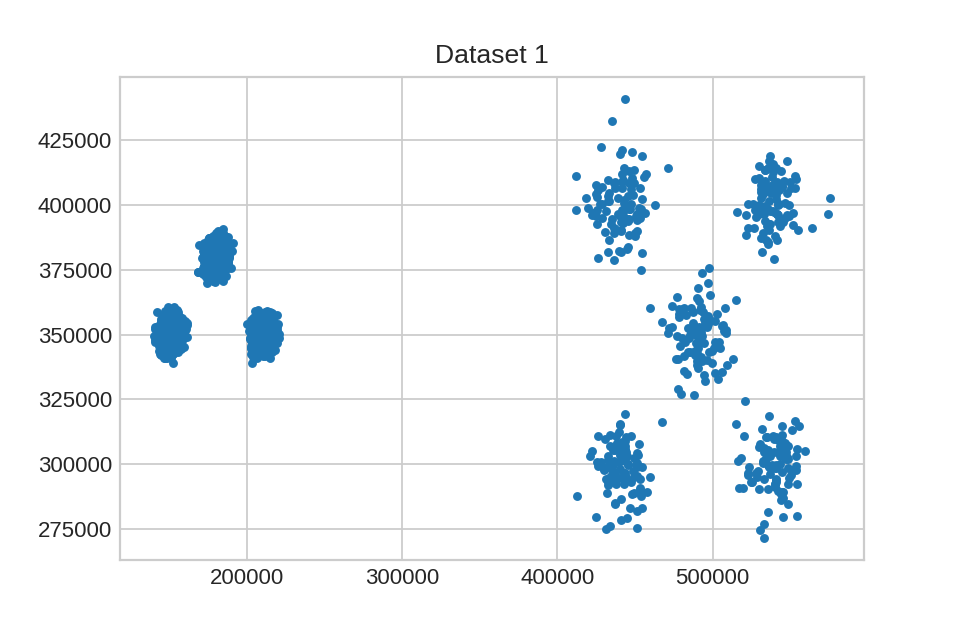
\includegraphics[scale=0.4]{experimentos/dataset1}
	\end{minipage}\qquad
	\begin{minipage}[t]{.3\textwidth}
		\centering
		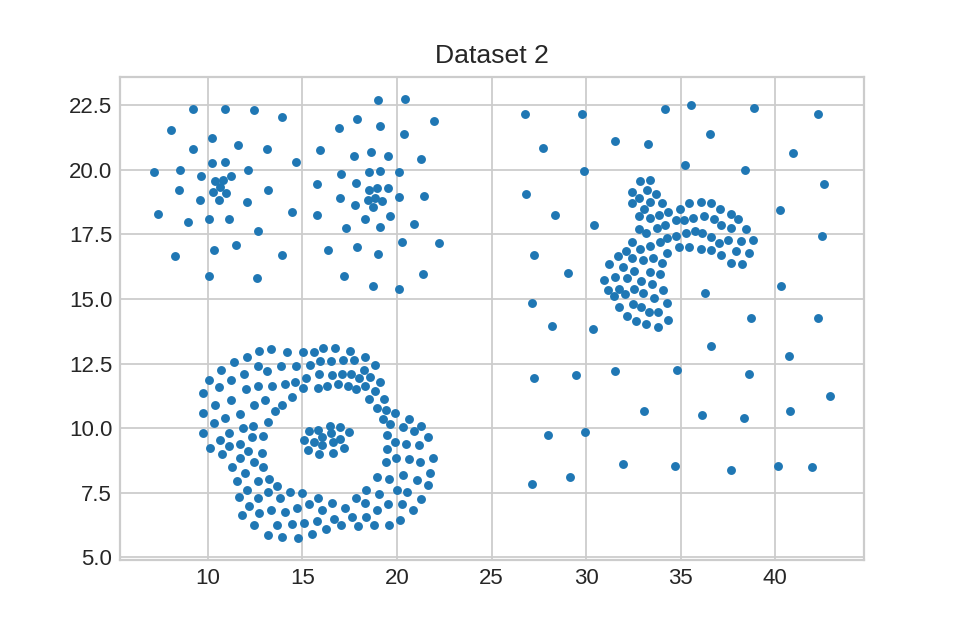
\includegraphics[scale=0.4]{experimentos/dataset2}
	\end{minipage}\qquad
	\begin{minipage}[t]{.3\textwidth}
		\centering
		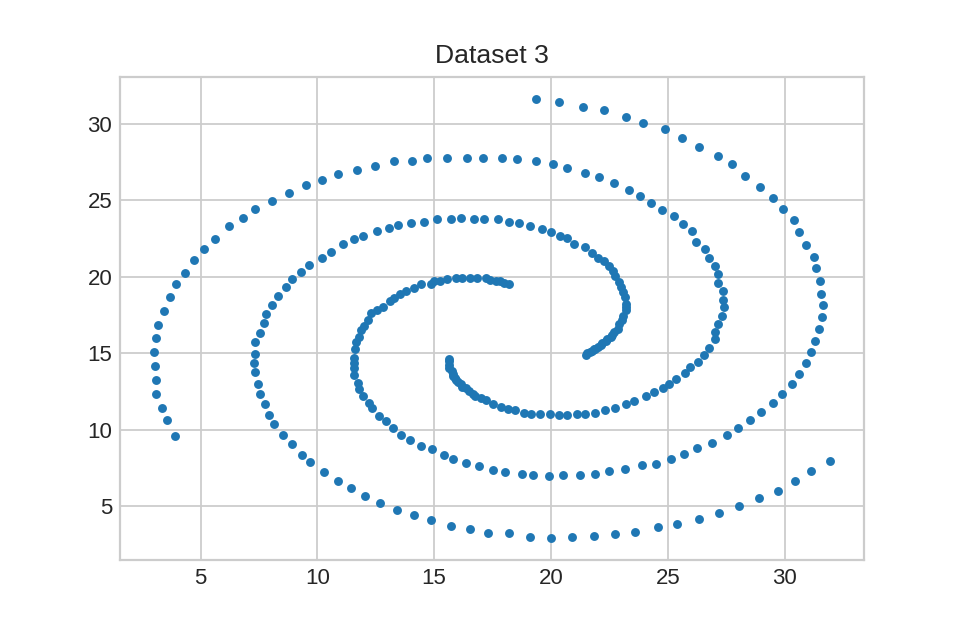
\includegraphics[scale=0.4]{experimentos/dataset3}
	\end{minipage}
\end{figure}	


\fbox{
	\parbox{0.9\textwidth}{
\textbf{Nota}: Para todos los criterios vamos a utilizar una profundidad de exploración fija de 9 ejes adyacentes. 
	}
}
\vspace{10 pt}

\subsubsubsection{Solo desvío estándar}
En este caso, vamos a descartar únicamente los ejes que son declarados inconsistentes al exceder en más de $\sigma$ veces el desvío estándar aplicado sobre el tamaño de eje promedio del vecindario.

\begin{figure}[H]
	\centering
	\begin{minipage}[t]{.3\textwidth}
		\centering
		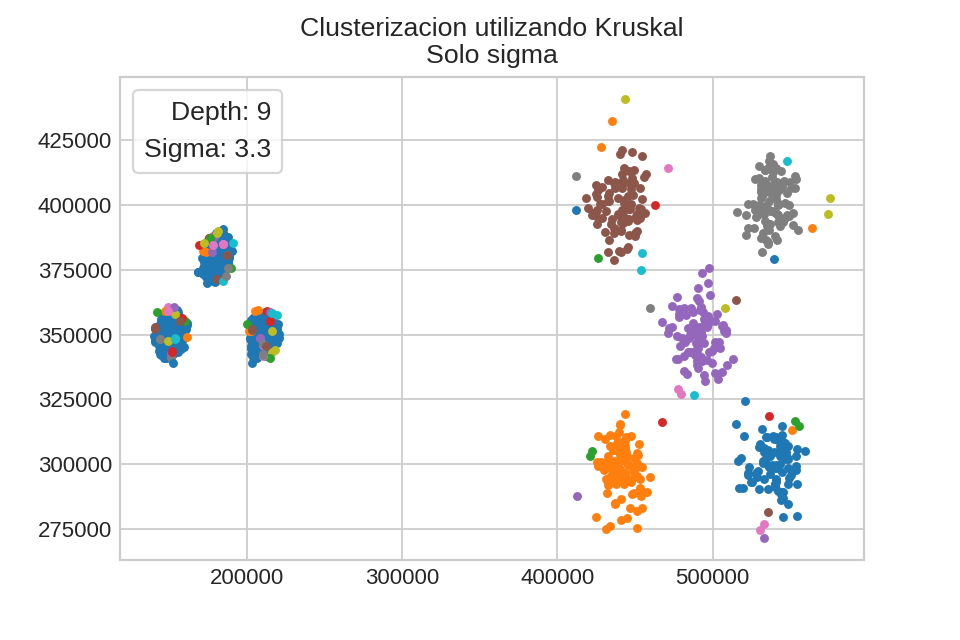
\includegraphics[scale=0.4]{experimentos/ds1-solosigma}
	\end{minipage}\qquad
	\begin{minipage}[t]{.3\textwidth}
		\centering
		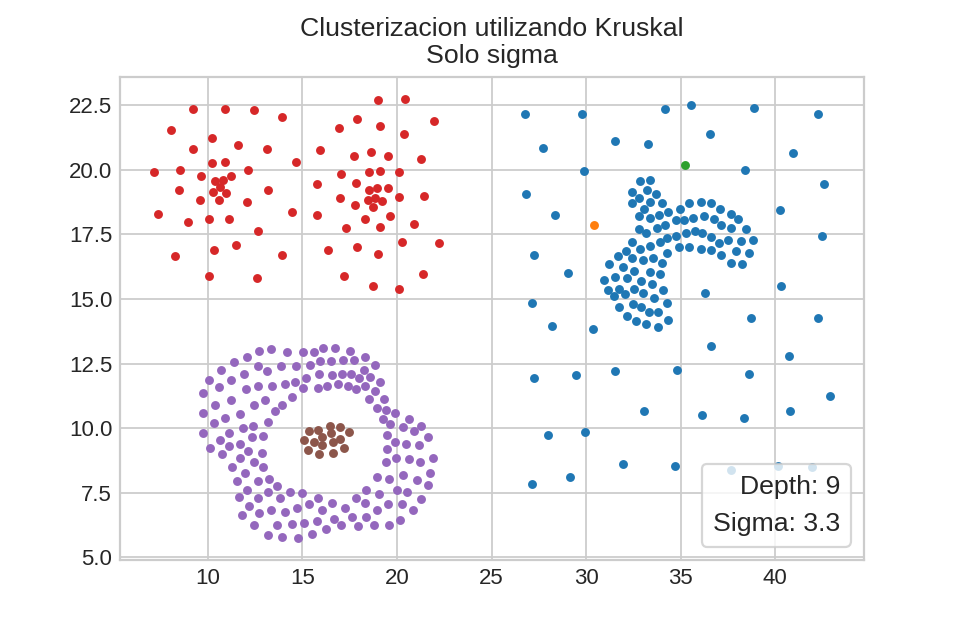
\includegraphics[scale=0.4]{experimentos/ds2-solosigma}
	\end{minipage}\qquad
	\begin{minipage}[t]{.3\textwidth}
		\centering
		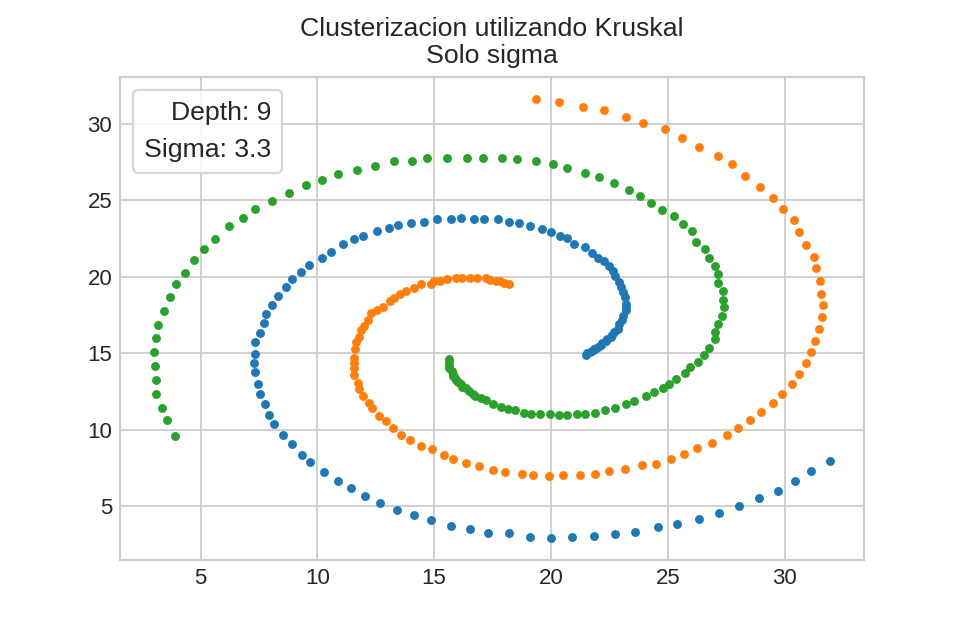
\includegraphics[scale=0.4]{experimentos/ds3-solosigma}
	\end{minipage}
\end{figure}	

Como podemos ver, utilizar solo el desvío estándar sirve para algunos casos, sin embargo tiene problemas para el \textit{dataset-1}, dado que en los clusters más chicos la desviación estándar entre los puntos es más alta, al estar todos más juntos. No podemos lograr un consenso de clusters sobre estos sin perjudicar la clusterización para los grupos de la derecha.


\subsubsubsection{Solo relación sobre el eje promedio}
En este caso, vamos a descartar únicamente los ejes que son declarados inconsistentes al ser $\digamma$ veces más grandes que el tamaño de eje promedio del vecindario.


\begin{figure}[H]
	\centering
	\begin{minipage}[t]{.3\textwidth}
		\centering
		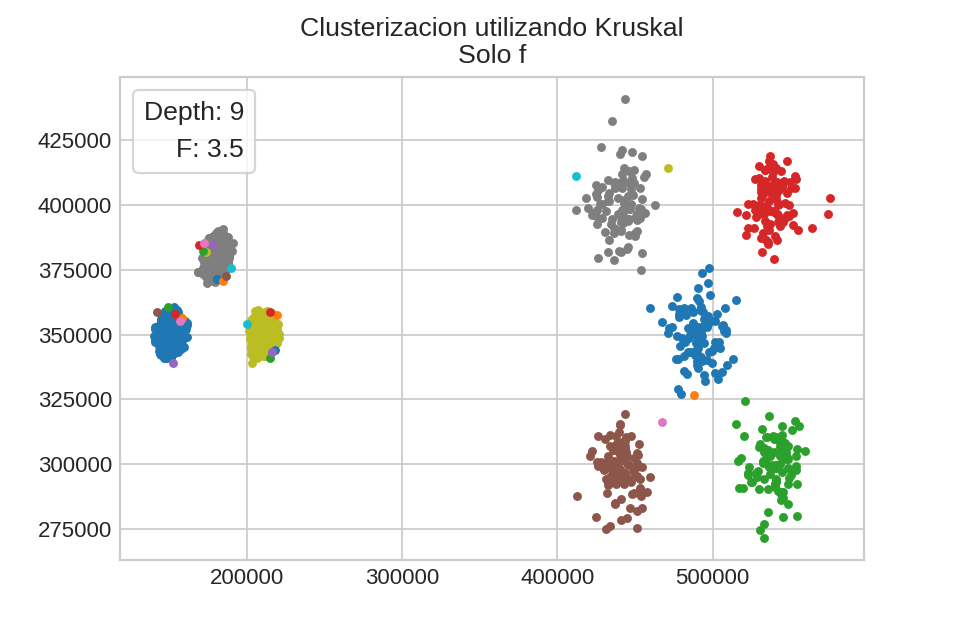
\includegraphics[scale=0.4]{experimentos/ds1-solof}
	\end{minipage}\qquad
	\begin{minipage}[t]{.3\textwidth}
		\centering
		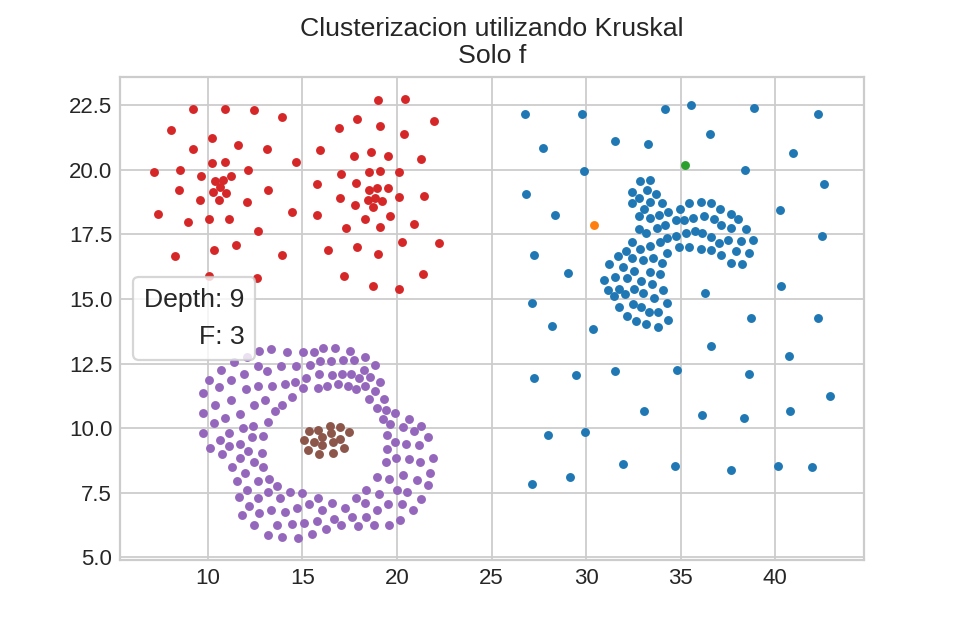
\includegraphics[scale=0.4]{experimentos/ds2-solof}
	\end{minipage}\qquad
	\begin{minipage}[t]{.3\textwidth}
		\centering
		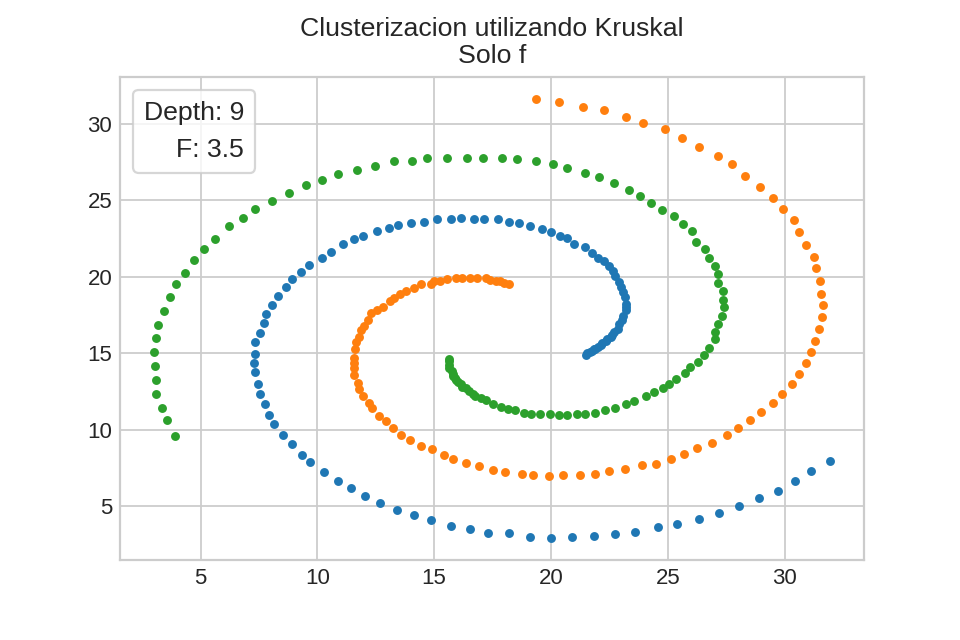
\includegraphics[scale=0.4]{experimentos/ds3-solof}
	\end{minipage}
\end{figure}

En este caso podemos ver que el \textit{dataset-1} no es problema para este criterio, aunque hay que notar que para el caso del \textit{dataset-2}, hubo que elegir un $f$ distinto, ya que los clusters de lado izquierdo eran agrupados con el valor utilizado para los otros datasets.

\subsubsubsection{Desvío estándar o relación de eje promedio}
Para este caso, los ejes inconsistentes van a ser los que cumplan con alguno de los dos criterios anteriores


\begin{figure}[H]
	\centering
	\begin{minipage}[t]{.3\textwidth}
		\centering
		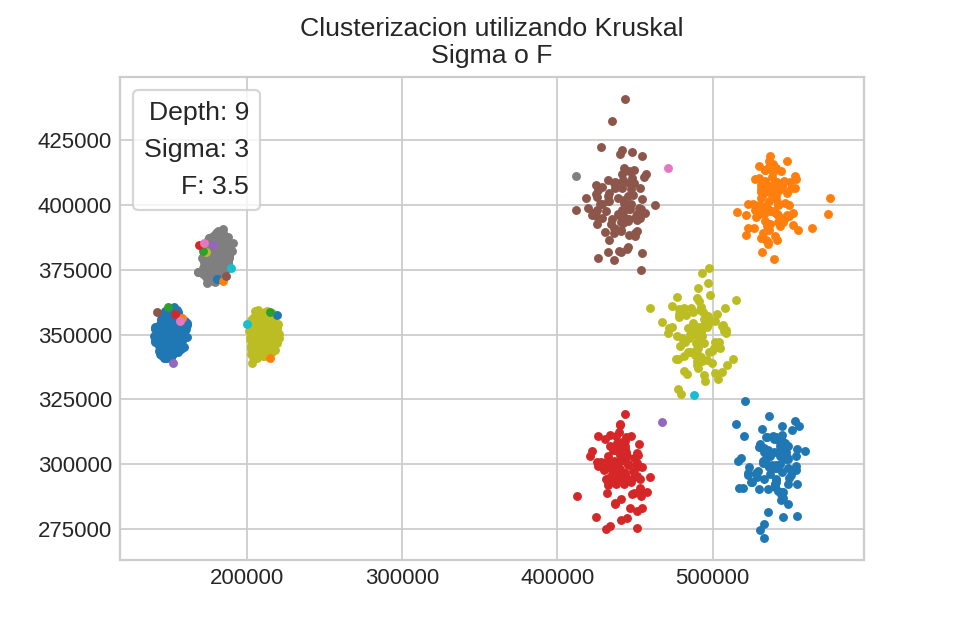
\includegraphics[scale=0.4]{experimentos/ds1-sigmaof}
	\end{minipage}\qquad
	\begin{minipage}[t]{.3\textwidth}
		\centering
		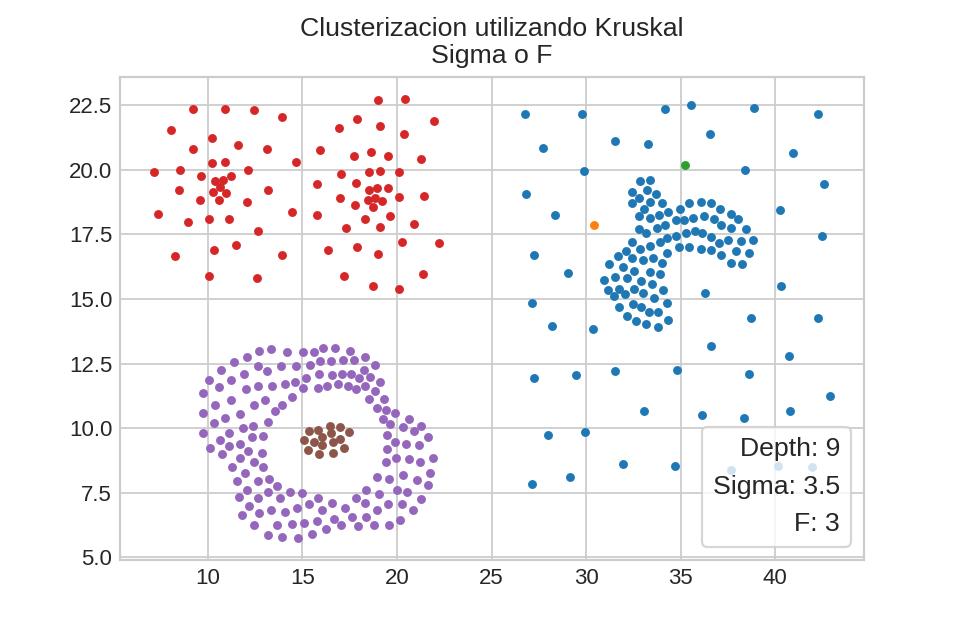
\includegraphics[scale=0.4]{experimentos/ds2-sigmaof}
	\end{minipage}\qquad
	\begin{minipage}[t]{.3\textwidth}
		\centering
		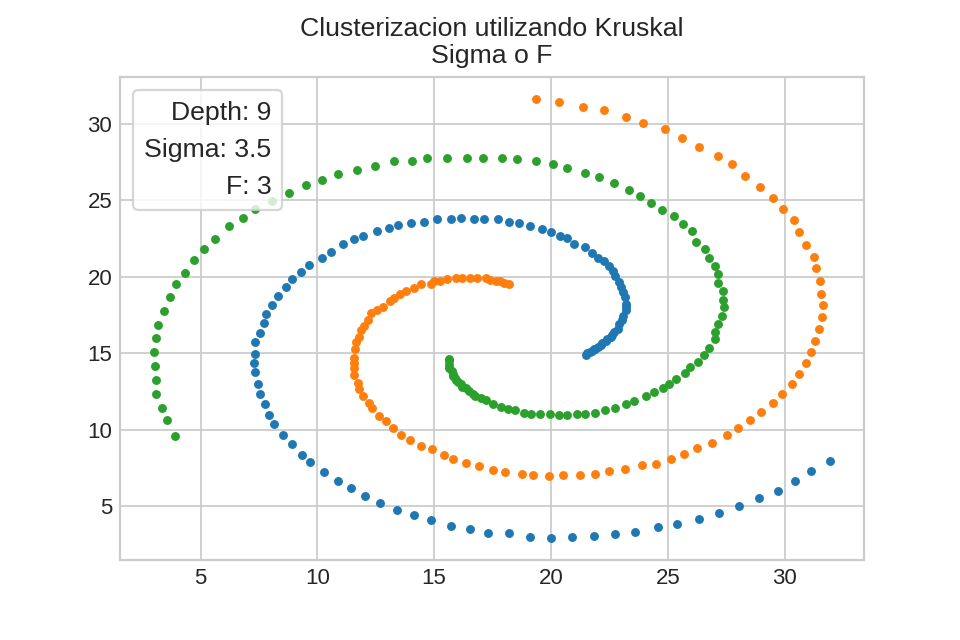
\includegraphics[scale=0.4]{experimentos/ds3-sigmaof}
	\end{minipage}
\end{figure}

Al utilizar cualquiera de los dos criterios anteriores para descartar nodos, podemos ver que en general toma precedencia el criterio por ‘f’ (relación de tamaño con el eje promedio). Por lo que no observamos beneficios al incluir el desvío estándar en la comparación. 

\subsubsubsection{Desvío estándar y relación de eje promedio}
Para este último caso, vamos a descartar únicamente los ejes que sean declarados inconsistentes tanto por el criterio del desvío estándar como por el criterio de relación de eje.

\begin{figure}[H]
	\centering
	\begin{minipage}[t]{.3\textwidth}
		\centering
		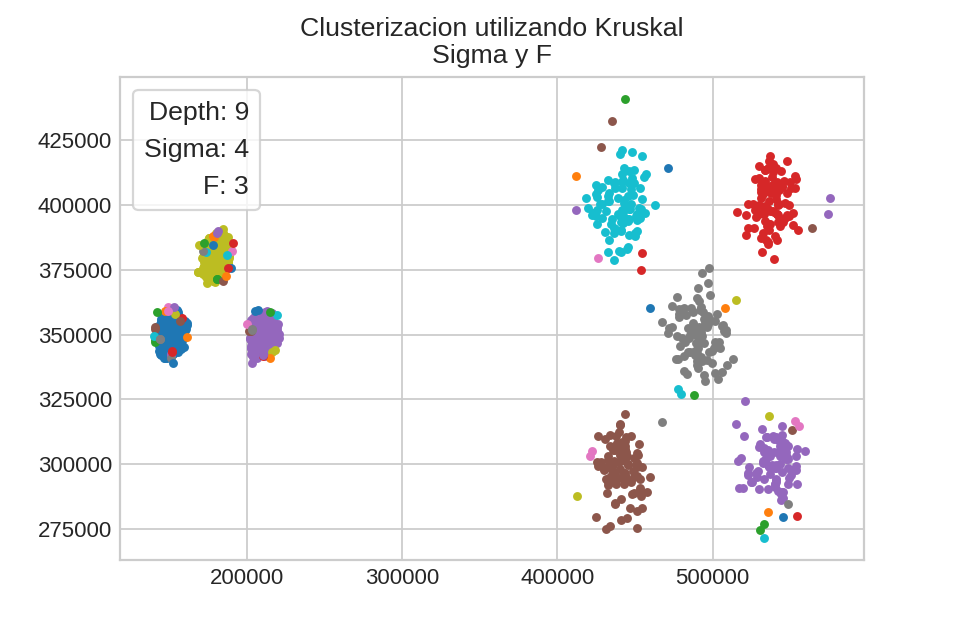
\includegraphics[scale=0.4]{experimentos/ds1-sigmayf}
	\end{minipage}\qquad
	\begin{minipage}[t]{.3\textwidth}
		\centering
		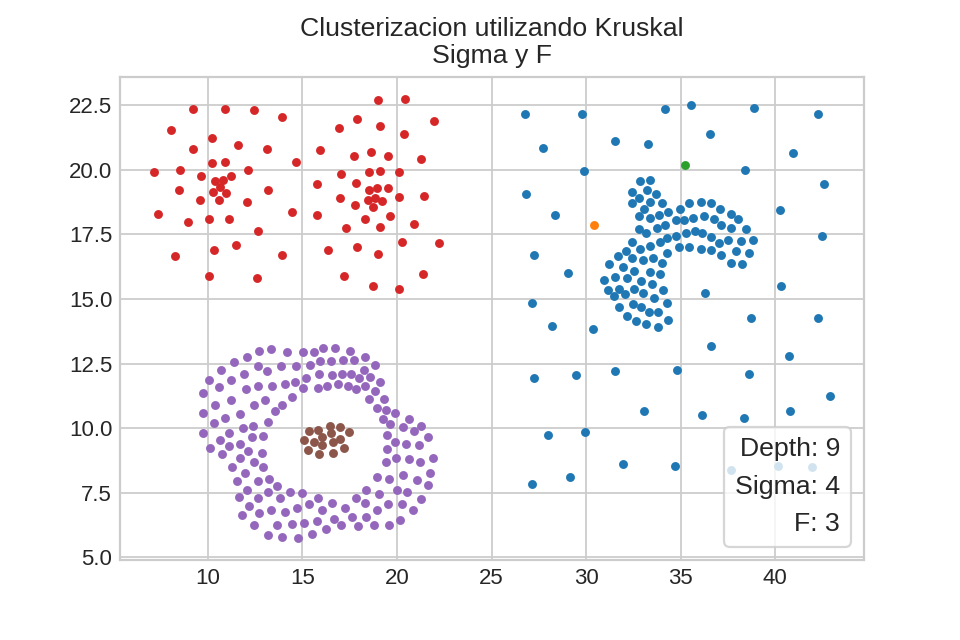
\includegraphics[scale=0.4]{experimentos/ds2-sigmayf}
	\end{minipage}\qquad
	\begin{minipage}[t]{.3\textwidth}
		\centering
		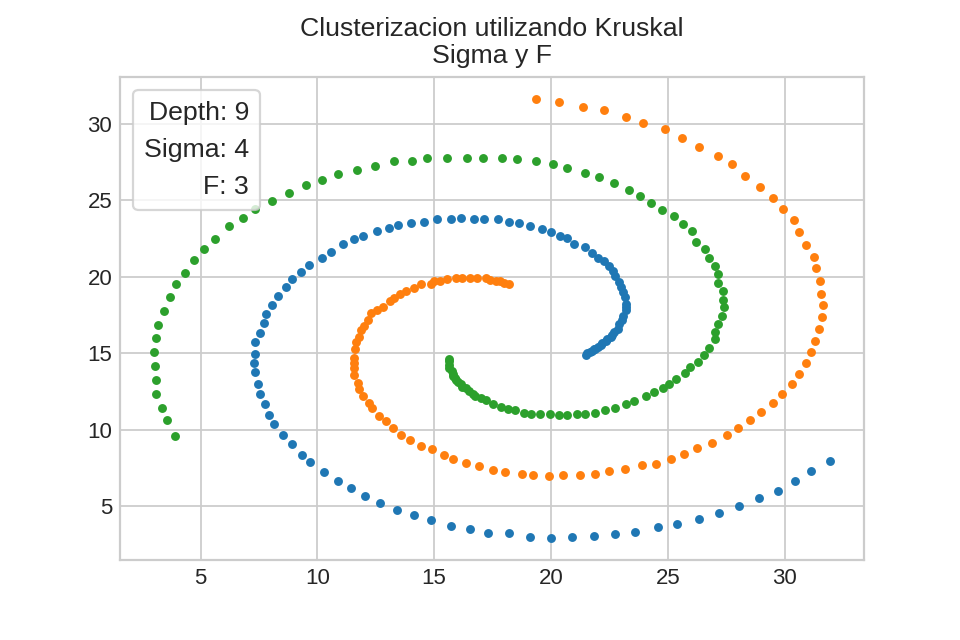
\includegraphics[scale=0.4]{experimentos/ds3-sigmayf}
	\end{minipage}
\end{figure}

Siguiendo el caso anterior, podemos ver que usar la conjunción sólo resulta en peores resultados, dado que para forzar la clusterización en algunos grupos, debemos usar un valor alto para sigma, lo cual resulta en agrupamientos indeseados en otras partes del grafo.

\subsubsubsection{Conclusiones}

Para los grafos elegidos para el experimento, resulta más conveniente utilizar únicamente la relación del eje contra el tamaño promedio de ejes. Como experimentos para profundizar, se deberían elegir grafos en los cuales la desviación estándar sea mayor al tamaño de eje promedio, en cuyo caso podríamos sacar provecho de combinar ambos criterios.


\subsubsection{Kruskal vs Kruskal con path compression}
Tal como fue presentado en la implementación del algoritmo de Kruskal, el mismo se puede implementar con un DSU con \textbf{path compression} que consiste en recordar el representante de un nodo buscado para poder accederlo en $\mathcal{O}(1)$ en la próxima consulta.

Para poder llevar a cabo dicha comparación, los escenarios planteados son representados con los siguientes grafos con 14600 puntos cada uno:

\begin{figure}[H]
	\centering
	\begin{minipage}[t]{.3\textwidth}
		\centering
		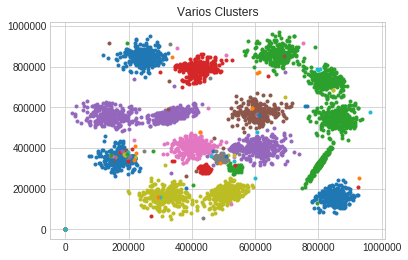
\includegraphics[scale=0.44]{experimentos/variosClusters}
	\end{minipage}\qquad
	\centering
	\begin{minipage}[t]{.3\textwidth}
		\centering
		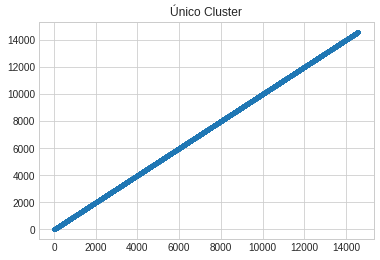
\includegraphics[scale=0.44]{experimentos/unicoCluster}
	\end{minipage}\qquad
\end{figure}	

\textbf{Nota}: Los puntos de la curva representan el promedio de ciclos de reloj de 10 ejecuciones por punto. Para cada grafo, desde 0 hasta 6500 se generaron datos en intervalos de 325 puntos, luego se genero información para 11500 puntos y por último para 14600 puntos.

\vspace{10 pt}

Los puntos a evaluar son:
\begin{itemize}
\item Performance entre Kruskal y Kruskal con path compression con varios clusters.
\item Performance entre Kruskal y Kruskal con path compression con un único cluster.
\item Evaluación de Kruskal con cota.
\end{itemize}


\subsubsubsection{Performance con varios clusters}


Al utilizar un grafo de 14600 puntos repartido en varios clusters como se pudo observar en la figura, se puede ver que cada cluster no contiene muchos puntos. Si bien, la alternativa de kruskal con path compression permite acceder al representante de un cluster en  $\mathcal{O}(1)$, al tratarse de clusters con pocos puntos, se espera que haya una diferencia mínima en los ciclos de reloj.

\begin{figure}[H]
	\centering
	\begin{minipage}[t]{.3\textwidth}
		\centering
		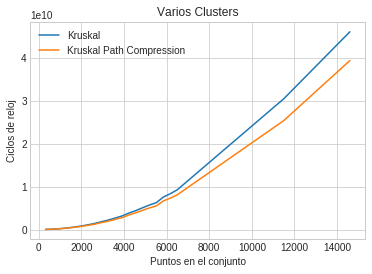
\includegraphics[scale=0.48]{experimentos/variosNormal}
	\end{minipage}
\end{figure}

Si bien la cantidad de ciclos de reloj entre una implementación y la otra comienzan a distanciarse a medida que se incrementan los puntos, la diferencia es mínima y se puede comprobar que la implementación con path compression se resuelve en menos ciclos.


\subsubsubsection{Performance con un único cluster}

Al utilizar el grafo de 14600 puntos repartido en un único cluster se espera que la optimización de path compression sea más visible y haya una mayor diferencia en la ejecución de cada algoritmo. 

\begin{figure}[H]
	\centering
	\begin{minipage}[t]{.3\textwidth}
		\centering
		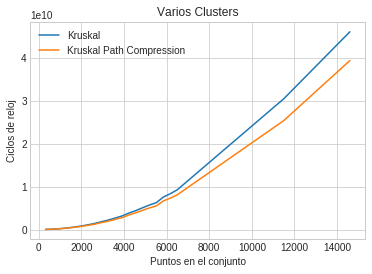
\includegraphics[scale=0.48]{experimentos/variosNormal}
	\end{minipage}
\end{figure}

Como se puede observar en la figura, los ciclos de reloj para cada algoritmo se distancian con una mayor diferencia que el caso anterior. Esto se debe a que la implementación normal de kruskal debe recorrer todo el arreglo de representantes, equivalente a recorrer todos los puntos ya analizados, para obtener el representante del cluster, que es único. En cambio, en el grafo anterior, los clusters contenían menos puntos, por ello la diferencia no era tan notable. En la última parte del grafo es posible ver como la pendiente de la ejecución para kruskal crece más rapidamente que para kruskal con path compression.


\subsubsubsection{Evaluación de cota}

La complejidad de ambas implementaciones es la misma, por eso se espera que ante la cota tomada, ambos pasen a estar por debajo de la misma a partir de un cierto valor.

\begin{figure}[H]
	\centering
	\begin{minipage}[t]{.3\textwidth}
		\centering
		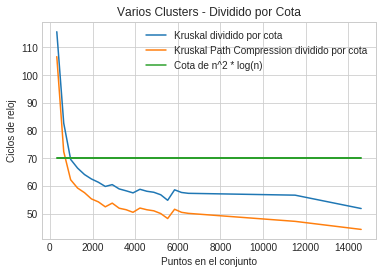
\includegraphics[scale=0.44]{experimentos/variosDivididoPorCota}
	\end{minipage}
	\centering
	\begin{minipage}[t]{.3\textwidth}
		\centering
		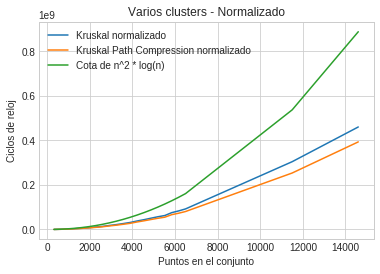
\includegraphics[scale=0.44]{experimentos/variosNormalizadoCota}
	\end{minipage}
\end{figure}

Como podemos ver, la funcion converge a un valor constante al dividirla por la complejidad planteada, lo cual demuestra que cumple con dicha cota.
\subsubsection{Comparacion de Kruskal contra Prim}

Al comparar Prim y Kruskal a la hora de clusterizar, podemos ver que ambos producen resultados similares. La diferencia entre ambos existe a la hora de generar el árbol generador mínimo, sobre el cual luego se descartan los ejes inconsistentes.

\begin{figure}[H]
	\centering
	\begin{minipage}[t]{.3\textwidth}
		\centering
		\includegraphics[scale=0.4]{experimentos/kvp-dataset-11-Kruskal}
	\end{minipage}\qquad
	\begin{minipage}[t]{.3\textwidth}
		\centering
		\includegraphics[scale=0.4]{experimentos/kvp-dataset-4-Kruskal}
	\end{minipage}\qquad
	\begin{minipage}[t]{.3\textwidth}
		\centering
		\includegraphics[scale=0.4]{experimentos/kvp-dataset-6-Kruskal}
	\end{minipage}
\end{figure}	

\begin{figure}[H]
	\centering
	\begin{minipage}[t]{.3\textwidth}
		\centering
		\includegraphics[scale=0.4]{experimentos/kvp-dataset-11-Prim}
	\end{minipage}\qquad
	\begin{minipage}[t]{.3\textwidth}
		\centering
		\includegraphics[scale=0.4]{experimentos/kvp-dataset-4-Prim}
	\end{minipage}\qquad
	\begin{minipage}[t]{.3\textwidth}
		\centering
		\includegraphics[scale=0.4]{experimentos/kvp-dataset-6-Prim}
	\end{minipage}
\end{figure}	

\subsubsubsection{Conclusiones}

Sin embargo, cabe destacar para Kruskal -al ser un algoritmo bottom up- armar los clusters una vez recortado el árbol generador mínimo es una tarea trivial, ya que el algoritmo se basa en formar clusters desconectados. En este aspecto, debemos realizar una solución Ad-Hoc para Prim, lo cual nos fuerza a obtener una complejidad mayor, a fuerza de no implementar Kruskal para clusterizar dentro de Prim.

\begin{figure}[H]
	\centering
	\begin{minipage}[t]{.45\textwidth}
		\centering
		\includegraphics[scale=0.55]{experimentos/prim-v-kruskal}
	\end{minipage}\qquad
	\begin{minipage}[t]{.45\textwidth}
		\centering
		\includegraphics[scale=0.55]{experimentos/prim-v-kruskal-acotado}
	\end{minipage}
\end{figure}	


\subsection{Conclusiones}

\subsubsection{Analisis Comparativo entre los Algoritmos} \label{analisisComparativo}

La problematica de arbitraje fue resuelta con los algoritmos de Bellman-Ford y Floyd-Warshall como mostramos en las secciones anteriores. Sabemos que la complejidad de Bellman-Ford es $\mathcal{O}(nm)$. Si tenemos en cuenta que en este problema de arbitraje necesitamos el camino minimo entre todo par de nodos, debemos ejecutar el algoritmo otras $`$n' veces, lo cual resulta en una complejidad de $\mathcal{O}(n^{2}m)$. Por otro lado, sabemos que la complejidad de Floyd-Warshall $\mathcal{O}(n^{3})$.

Esto nos dice que Bellman-Ford no tiene un buen caso en grafos completos, que es el caso del arbitraje. Floyd-Warshall no es afectado por grafos completos, pero si por el tamaño del mismo. Esto tiene relevancia dado que la experimentación ejecutada mostraba al algoritmo de Floyd como un claro ganador en tiempo. Es cierto que la implementación de Bellman-Ford no esté en el $\%$100 de su efectividad, pero es de esperar que en un grafo completo, Floyd-Warshall se comporte mejor.

Con respecto a los casos donde puede convenir uno u otro, vimos que ambos pueden ser utilizados para detectar un ciclo negativo. Floyd-Warshall es superior si el arbitraje se encuentra entre los primeros nodos, Bellman-Ford si no lo hay.

\end{document}

